\chapter{A contrastive study of NLM's syntactic abstraction based on long-distance agreement
} \label{chp:main_project}
\vspace{-1.3cm}  

\startcontents[chapters]
\printmyminitoc{
}
This chapter, forming the centerpiece of this dissertation, builds directly upon the studies reviewed in Chapter \ref{chp:NA_tasks}. We expand previous research by conducting a contrastive analysis of a Transformer model through two carefully crafted long-distance agreement tasks in French. We aim to investigate how well the Transformer can handle these two strucutre-sensitive phenomena, and whether its performance stems from its ability to build an abstract, high-level (maybe hierarchical) sentence representation~\citep{giulianelli-etal-2018-hood,lakretz-etal-2019-emergence} or merely because it captures surface statistical regularities, as suggested by previous studies~\citep{sennhauser-berwick-2018-evaluating, chaves-2020-dont,li-wisniewski-2021-neural}. To effectively evaluate the model's syntactic capacity, we first introduce a novel heuristic-based evaluation protocol, which enables us to probe the model's ability to handle agreement tasks beyond superficial heuristics. We then use probing approaches, paired with causal analysis, to identify the location of the syntactic information within the model and determine how the model actually uses this information for agreement resolution. 


\paragraph{Chapter outline} This chapter is structured as follows:
Section \ref{sec:intro_main_project} introduces the research question and relevant background concepts, as well as the two agreement tasks that are central to our study. In Section \ref{sec:heuristics}, we revisit the number agreement tasks through a heuristic-based evaluation protocol to address potential confounding factors. These refined tasks and the evaluation protocol serve as the foundation for all subsequent experiments outlined in this chapter. In Section \ref{sec:probing_location}, we investigate the specific location of syntactic information within the autoregressive Transformer language model. Following this, Section \ref{sec:causal} analyses how the model uses this encoded syntactic information to process long-distance agreement phenomena. In Section \ref{sec:word_order_NA}, we explore the relationship between the model's ability to abstract syntactic structure and the sequential word order information presented in the input sequences. The chapter concludes with Section \ref{sec:conclu_main_projct}, where we recapitulate our findings and discuss their implications.

\section{Introduction} \label{sec:intro_main_project}

Transformers-based language models~\citep{NIPS2017_3f5ee243,devlin-etal-2019-bert,brown2020language} have reshaped NLP with their unparalleled performance across a wide range of language tasks. Their empirical success, coupled with the findings of previous studies (see Section \ref{sec:review_structure_nlm}), indicates that these models potentially have acquired a certain level of abstraction in understanding language structure. Since~\cite{linzen-etal-2016-assessing}, the long distance agreement task has been a paradigmatic test for assessing the ability of NLMs to uncover syntactic information from raw texts: a model able to predict the long-distance agreement dependency, has to, to some extent, develop an abstract representation of the syntactic structure and encode it in its internal representations.   

In this study, we investigate how Transformer language models process and represent syntactic structure through long-distance agreements tasks. The essential research question we aim to explore is: When resolving long-distance agreements, to what extent do models abstract their representations from surface pattern recognition, and are they able to develop meaningful, syntactically driven representations of linguistic structure? 

By addressing this question, we can evaluate model's representational adequacy for modeling syntactic structures and develop linguistically-informed analysis tools to enhance our understanding and control over these models. Such insights are crucial for evaluating these models as potential explanatory explanatory models for human language processing. Moreover, delving into the linguistic abstraction of these models can provide insight into the properties that contribute to the success of NLMs but also identify their limitations, which could help guide the creation of more effective architectures. For instance, previous studies find that modeling explicitly hierarchical structure as an inductive bias of RNN models helps them learn structure-sensitive phenomena more effectively~\citep{kuncoro-etal-2018-lstms,wilcox-etal-2019-structural}. Despite the remarkable empirical success of Transformer-based models, they can be fragile, especially when faced with noisy or adversarial inputs~\citep{wang2022bert}. Integrating human linguistic priors into these models might provide added robustness and optimize learning efficiency~\citep{lake2017building,besold2017neuralsymbolic}.


To explore this question, we focus on two types of number agreement phenomena in French, both feature morphological markings:
\begin{exe}
   \ex\label{ex:agrS}
   \gll Les \textbf{chat·s} [ que Noûr aime bien
  ]\textcolor{blue}{$_{RC}$} \textbf{jou·ent} dans le jardin.   \\
   {\fontsize{9}{11}\selectfont The\_Pl} {\fontsize{9}{11}\selectfont cats\_\textbf{Pl}} {\fontsize{9}{11}\selectfont [} {\fontsize{9}{11}\selectfont that} {\fontsize{9}{11}\selectfont Noûr} {\fontsize{9}{11}\selectfont likes\_Sg} {\fontsize{9}{11}\selectfont a\_lot} {\fontsize{9}{11}\selectfont ]$_{RC}$} {\fontsize{9}{11}\selectfont play\_\textbf{Pl}} {\fontsize{9}{11}\selectfont in} {\fontsize{9}{11}\selectfont the } {\fontsize{9}{11}\selectfont garden.} \\
   \ex\label{ex:agrO}
  \gll Les \textbf{chat·s} [ que Noûr a \textbf{adopté·s} ]\textcolor{blue}{$_{RC}$} sont mignons. \\
   {\fontsize{9}{11}\selectfont The\_Pl} {\fontsize{9}{11}\selectfont cats\_\textbf{Pl}} {\fontsize{9}{11}\selectfont [} {\fontsize{9}{11}\selectfont that} {\fontsize{9}{11}\selectfont Noûr} {\fontsize{9}{11}\selectfont has} {\fontsize{9}{11}\selectfont adopted\_\textbf{Pl}} {\fontsize{9}{11}\selectfont ]$_{RC}$} {\fontsize{9}{11}\selectfont are\_Pl} {\fontsize{9}{11}\selectfont cute\_Pl} \\
\end{exe}
Example (\ref{ex:agrS}) demonstrates a subject-verb agreement between the noun ``chats'' and the main verb ``jouent'' across a relative clause, while (\ref{ex:agrO}) showcases an object-past participle agreement between the same noun ``chats'' and the past participle ``adoptés''. At first glance,
(\ref{ex:agrS}) and (\ref{ex:agrO}) may appear to represent
identical agreements between a noun and a verbal form separated by a
few words. Yet from a linguistic perspective they are substantially different: while the former involves the subject controlling the main verb's number, the latter involves anaphora resolution and movement---operations that are fundamentally different from the phrase structure embedding in the subject-verb agreement (see \S\ref{sec:two_agreements} for more detailed description). 

It is unclear whether
and how a Transformer language model can identify these abstract
representations based merely on the words sequence. The present work aims to contrast how Transformer handles these two kinds of
agreement. Specifically, we seek to determine whether the Transformer LM encodes the \textbf{same}
abstract structure in its internal representations to capture the
information required for agreement resolutions, or if it instead encodes an abstract structure that reflects the
\textbf{distinction} made in the theoretical modeling of these two
agreements. This contrast will shed new light on our understanding
of the internal workings of Transformer models.


This chapter offers two key contributions.
First, we expand the existing syntactic evaluation paradigm by conducting a contrastive analysis of a Transformer model's ability to abstractly represent two superficially similar syntactic phenomena in French: long-distance subject-verb agreement and a less studied phenomenon, object-past participle agreement. 
Second, we introduce an integrated linguistically-informed analysis framework that can serve as a template for empirically testing linguistic or cognitive theories with computational models. 

As an initial step, we introduce a novel heuristic-based evaluation protocol to revisit conventional number agreement tasks. This helps to discern whether the model relies on structural patterns or surface-level heuristics. Our findings indicate that Transformer models excel at both agreement tasks, successfully abstracting away from potential lexical or heuristic confounds. Subsequently, we use probing classifiers and causal intervention on self-attention to examine
\textbf{where} the Transformer model encodes syntactic information internally and \textbf{how} the model uses it in agreement resolution tasks. The results reveal that for both phenomena, even though the long-distance
agreement information is mainly encoded locally across the tokens
between the two agreeing elements, Transformer model deploys distinct, linguistically motivated strategies to process each phenomenon. Lastly, through ablation studies, we explore the role of positional embeddings in the Transformer's architecture. 


\section{Revisiting number agreement tasks via a heuristic-based evaluation protocol} \label{sec:heuristics}

As discussed in Chapter~\ref{chp:NA_tasks}, many recent studies have demonstrated that unsupervised sentence representations generated by neural language models encode syntactic information, as evidenced by their success in predicting long-distance agreements. However, conventional behavioral assessments, which focus solely on output, fall short of determining whether a model's success in these tasks arises from genuine syntactic understanding or from exploiting superficial patterns in the data.

To address this issue, we introduce a heuristic-based evaluation protocol tailored for agreement tasks.  This protocol enables us to identify cases where the correct answer cannot be inferred through simple surface-level heuristics. If the model still performs well under these conditions, it would strongly suggest that it has indeed acquired a level of non-superficial syntactic competence.
We further complement this with control experiments aimed at assessing other confounding factors that might influence the model's predictions. This multi-faceted evaluation strategy lays the groundwork for the subsequent development and assessment of different interpretation techniques, as we will explore in Sections \ref{sec:probing_location} and \ref{sec:causal}.

\subsection{Syntactic phenomena} \label{sec:two_agreements}

In this study, we extend the agreement predictions approach to non-English languages by considering French, a morpho-syntactically richer language. Unlike English, where agreement is primarily limited to subject-verb pairs in the third person, singular present tense, French exhibits a wider range of agreement features, including gender and number agreement across various grammatical categories like adjectives, pronouns, articles, and past participles. This complexity provides a richer testing ground for exploring the syntactic capabilities of neural language models.



The number agreement tasks in our study address two agreement phenomena: subject-verb agreement across relative clauses (henceforth \textit{S-V agreement}) and object-past participle agreement (henceforth \textit{O-PP agreement}) in French. In the following sections, for both types of agreement we refer to the noun item providing the agreement information the \textbf{cue}, and the verbal item as the \textbf{target}. We focus exclusively on sentences involving \emph{object relatives} such as those analyzed in Figure~\ref{fig:ex_agreement}, where the words that intervened between the \textit{cue} and the \textit{target} contain at least one relative clause. Despite the superficial similarities between the two phenomena --- both featuring a relationship between a noun and a verbal form separated by a few words containing relative clause elements --- they receive significantly different linguistic analyses.

\begin{figure*}[!ht]
  \centering
  \begin{subfigure}[b]{\textwidth}
    \centering
    \begin{dependency}
      \tikzstyle{POS}=[font=\fontsize{9}{11}\selectfont]
      %\tikzset{POS/.style={font=\fontsize{9}{11}\selectfont}}
      \begin{deptext}
        \textbf{Les} \& \textbf{chat·s} \& dans \&  le \& \underline{jardin} \& que \& \underline{Marie} \& nourrit \& régulièrement \_\_ \&\textcolor{red}{miaul·ent} \& .\\
         |[POS]| The\_Pl \& |[POS]| cats\_Pl \& |[POS]| in \& |[POS]| the \& |[POS]| garden\_Sg \& |[POS]| that \& |[POS]| Marie \& |[POS]| feeds \& |[POS]| regularly \&|[POS]| meow\_Pl \& |[POS]| . \\
          \& {\bf cue} \&  \&  \&  \&  \& \& \&   \& \textcolor{red}{\bf target} \&  \\
      \end{deptext}
      %\depedge[edge unit distance=0.5ex,blue]{2}{6}{antecedent}
      %\depedge[edge unit distance=0.5ex,blue]{6}{9}{object}
      \depedge[edge unit distance=0.5ex,red]{10}{2}{nsubj}
    \end{dependency}
    \caption{Example of subject-verb agreement}
    \label{fig:ex-subj-v}
    \end{subfigure}%
  
  \vspace{0.5cm}
  \begin{subfigure}[b]{\textwidth}
    \centering
    \begin{dependency}
      \tikzstyle{POS}=[font=\fontsize{9}{11}\selectfont]
      \begin{deptext}
        \textbf{Les} \& \textbf{chat·s} \& dans \&  le \& \underline{jardin} \& \textcolor{blue}{que} \& \underline{Marie} \& a \& \textcolor{blue}{adopté·s} \_\_ \&miaulent .\\
         |[POS]| The\_Pl \& |[POS]| cats\_Pl \& |[POS]| in \& |[POS]| the \& |[POS]| garden\_Sg \& |[POS]| that \& |[POS]| Noûr \& |[POS]| has \& |[POS]| adopted\_Pl \&|[POS]| meow\_Pl \& |[POS]| . \\
          \& {\bf cue} \&  \&  \&  \&  \& \& \& \textcolor{blue}{\bf target}  \&  \&  \\
      \end{deptext}
      \depedge[edge unit distance=0.5ex,blue]{2}{6}{antecedent}
      \depedge[edge unit distance=0.5ex,blue]{6}{9}{object}
      %\depedge[edge unit distance=1.0ex,red]{10}{2}{nsubj}
    \end{dependency}
    \caption{Example of object-past participle agreement}
    \label{fig:ex-obj-pp}
  \end{subfigure}
  \caption{In (a), the number of the main verb (\textit{miaulent}, in red) is determined by the head of the subject \textit{chats}.  In (b), the past participle in the relative clause (\textit{adopté}, in blue) has to agree in gender and number with its object (also in blue) when the latter precedes the verb. }.
  \label{fig:ex_agreement}
\end{figure*}


The subject-verb agreement across relative clauses is a case that clearly necessitates hierarchical representation. In (\ref{fig:ex-subj-v}), the main verb \textit{miaulent} (meow) must agree in number with its syntactic subject \textit{chats} (cats), regardless of the intervening elements. The relative pronoun \textit{que} (that) and the entire embedded clause are not relevant for determining the form of the main verb. The model needs to distinguish the main clause subject (\textit{chats}) from the embedded subject (\textit{Marie}) and ignore irrelevant attractors like \textit{jardin}. This requires a nuanced representation of clause-specific syntax and verb argument structure.

Compared to subject-verb dependency, the agreement of the past participle in object relative clauses relies on an abstract set of relations
between words occurring in different clauses. In French, the past participle conjugated with the auxiliary \textit{avoir} (have) in compound tenses, such as passé composé, must agree in number and gender with the direct object that precedes it.\footnote{Although in standard French, normative grammars indicate object-past participle agreement under wh-movement as obligatory, it in fact appears to be optional in colloquial French, where the past participle is often produced in its default form, which, in French, corresponds to the singular, masculine form of the participle ~\citep{belletti2017past}. Please refer to \textsection\ref{sec:heuristic_exp_setup} for a relevant analysis of the training data used in this study.} As shown in Figure~\ref{fig:ex-obj-pp}, the past participle within relative clause agrees in number and gender with its complement (the \cue) in the main clause, because the latter moves before it. Specifically, when agreement is required, a \texttt{-s} suffix (resp.\
\texttt{-e}) is added to the singular masculine form for plural objects
(resp.\ feminine). This agreement resolution involves an anaphora (indicated by the \textit{antecedent} arc)
and a filler-gap dependency. The filler is \textit{que} (that) and the gap, indicated with an underscore in Figure~\ref{fig:ex_agreement}, is an empty syntactic position licensed by the filler~\citep{kayne1989facets}. In the example~(\ref{fig:ex-obj-pp}), the relative pronoun
\textit{que} is the pre-verbal direct object of the past participle
\textit{adoptés} and triggers the agreement of the
past participle. To obtain its agreement features, the relative
pronoun has to be linked by anaphora to its nominal antecedent
\textit{chats}. In other words, to correctly agree the past participle
in theory, it is necessary to identify the object relative pronoun \textit{que} and
its antecedent. Additionally, the model has to ignore the effect of attractors
occurring between the antecedent of the relative pronoun and the past
participle. 


We only consider number agreement as \textit{i)} number
agreement is the only feature shared by the two agreements we
consider;\footnote{In French, the verb has to agree in number with its
  subject, and the past participle conjugated with the auxiliary
  \textit{avoir} agrees in number \emph{and} in gender with its direct object
  if the latter appears before it.}  \textit{ii)} the main purpose is to
design reasonably simple patterns allowing to extract a
sufficiently large number of representative examples. These restrictions allow us to carry out a fine-grained contrastive
analysis of NLMs ability to extract syntactic generalizations
from non-annotated corpora (\textsection\ref{sec:h_eval_protocol}).


\subsection{Datasets construction} \label{sec:NA_data}

As discussed in Chapter~\ref{chp:NA_tasks}, common approaches for creating challenge sets typically rely on template-based generation or extraction from gold parses. Template-based synthetic data, similar to the artificial stimuli employed in human linguistic experiments, provides controlled testing grounds. Yet, they may lack ecological validity and the variability of natural language. For example, our Transformer language model, trained on French Wikipedia text, achieved a perplexity score of 27. However, the score rises to 308 for materials from human experiments on French object-past participle agreement used in \cite{villata2017intervention}, and increases to 654 on a synthetic corpus for French subject-verb agreement across relative clauses from \cite{mueller-etal-2020-cross}. This score discrepancy highlights the potential detachment of synthetic data from the natural linguistic landscape, which could, in turn, affect the assessment of model capabilities. On the other hand, while gold parses from existing treebanks ensure accuracy, they may not provide a sufficient number of syntactically challenging examples. For instance, only 41 sentences were available for English in the study by \cite{gulordava-etal-2018-colorless}. 

To overcome these limitations, we adopt an approach focusing on naturally occurring sentences. This approach not only respects the ecological validity, but also reflects the complexity and diversity inherent in natural language. By extracting our target sentences from a large automatically parsed corpus, we collect a substantial and varied set of test items. Furthermore, we conduct a qualitative evaluation of our automatic parsing and extraction pipeline to guarantee the quality of the evaluation sets.

\paragraph{Overview} To construct the evaluation datasets for the number agreement tasks we consider, sentences were automatically extracted from the
French part of Project Gutenberg,\footnote{\url{https://www.gutenberg.org/}} which contains over 8 million sentences. We used
the French dependency parser~\citep{grobol-crabbe-2021-analyse} along with
pretrained French model from \textit{spaCy}~\citep{spacy} to parse the corpora,\footnote{The parser by~\cite{grobol-crabbe-2021-analyse} annotated only the part-of-speech tags and dependency relations, \textit{spaCy} supplemented these annotations with morphological features.} from which examples of target agreement phenomena were extracted using simple rules (detailled in the following paragraph).  This resulted in two evaluation sets: one for \ac{O-PP agreement}, consisting of 68,794 sentences (65\% with a singular \target and 35\% with a plural one), and spanning 837 past participle lemmas and 2,489 word forms. Another for \ac{S-V agreement} across relative clauses, consisting of 27,582 sentences (70\% with a singular \target 30\% with a plural one), and spanning 536 verb lemmas and 1533 verb forms. Both sets consist of sentences including at least one object relative clause between the \cue and \target. There are fewer items in the S-V agreement set because noun phrases modified by relative clause(s) occur more frequently in the object position than in the subject position of the main clause. In these two
evaluation sets, an arbitrary number of words can occur between the
\cue and \target: an average of five tokens occur between the antecedent and the past participle, and 11 tokens between the head of the
subject and the main verb. These “intervening” tokens include varied
constructions such as prepositional phrases, participials, or nested
relative clauses, which can pose additional challenges for agreement tasks. See Section~\ref{app:sample_sents} in the Appendix for sample sentences from the two evaluation sets. Note that in all our experiments, we ensure that the evaluation sets were completely separate from models training data.


\begin{figure*}[!ht]
  \centering
  \begin{subfigure}[b]{\textwidth}
    \centering
    \begin{dependency}
      \tikzstyle{POS}=[font=\fontsize{9}{11}\selectfont]
      \begin{deptext}
       \& \& NOUN \& PRON \&  \&VERB  \& \& VERB \&  \&  \&  \&    \\
        \& Les \& {\bf chat·s} \& {\bf que} \& Noûr \& aime \& bien \& {\bf jou·ent} \& dans \& le \& jardin \& . \\
       \& |[POS]| The\_Pl \& |[POS]| cats\_Pl \& |[POS]| that \& |[POS]| Noûr \& |[POS]| loves \& |[POS]| well \& |[POS]| play\_Pl \& |[POS]| in \& |[POS]| the \& |[POS]| garden\_Sg \& . \\
       \& \& {\bf cue} \&  \&  \&  \& \& {\bf target} \&  \&  \&  \&    \\
      \end{deptext}
      \depedge[edge unit distance=0.8ex]{8}{3}{nsubj}
      \depedge[edge unit distance=0.5ex]{4}{6}{object}
    \end{dependency}
    \caption{Example of the extraction pattern for subject-verb agreement across relative clauses}
    \label{fig:ex-subj-v_extraction}
  \end{subfigure}
  
  \vspace{0.5cm}
  
  \begin{subfigure}[b]{\textwidth}
    \centering
    \begin{dependency}
      \tikzstyle{POS}=[font=\fontsize{9}{11}\selectfont]
      \begin{deptext}
        \& \&  \&   \& NOUN \&  \&   \&  \& PRON \&  \&  \& VERB  \&  \\
       \& Il \& aime \&  les \& {\bf chat·s} \& dans \&  le \& jardin \& {\bf que}  \& Noûr \& {\bf a} \& {\bf adopté·s}  \& . \\
       \& |[POS]| He \& |[POS]| loves \& |[POS]| the\_Pl \& |[POS]| cats\_Pl \& |[POS]| in \& |[POS]| the \& |[POS]| garden\_Sg \& |[POS]| that \& |[POS]| Noûr \& |[POS]| has \& |[POS]| adopted\_Pl \& |[POS]| . \\
       \& \&  \&   \& {\bf cue} \&  \&   \&  \&  \&  \&  \& {\bf target}  \&  \\
      \end{deptext}
      \depedge[edge unit distance=0.5ex]{5}{12}{acl:relcl}
      \depedge[edge unit distance=0.5ex]{12}{9}{object}
    \end{dependency}
    \caption{Example of the extraction pattern for object-past participle agreement  }
    \label{fig:ex-obj-pp_extraction}
  \end{subfigure}
  \end{figure*}
\paragraph{Extraction procedure} The extraction rules used to construct evaluations datasets are based on the predicted dependency structure and morphological information of sentences. As illustrated in Figure \ref{fig:ex-subj-v_extraction}, for subject-verb agreement, a valid example must include a \textsc{Noun} and \textsc{Verb} connected by a \textit{nsubj} dependency and at least one relative pronoun \textit{que} acting as a direct object between them. For object-past participle agreement, as shown in Figure \ref{fig:ex-obj-pp_extraction}, a valid example has to include a
\textsc{Noun} and \textsc{Verb} connected by an \textit{acl:relcl}
dependency, with a direct object \textit{que} preceding the \textsc{Verb}, and the
auxiliary used by the target \textsc{Verb} must be \textit{avoir}
(to have). 

  
In the next step, we filtered out sentences containing ambiguous or non-agreement \target-\cue pairs. Based on syntactic-morphological information, we excluded
sentences that involved the \cue being part of a coordination structure, such as example (1) in Figure~\ref{fig:ex_test_set}, and those with number-ambiguous \cue or \target, including collective nouns or nouns and verbs with identical singular and plural forms.\footnote{We filtered out nouns with endings in \texttt{-s,-x,-z} and past-participles that ends with \texttt{-s}, as these forms often remain the same in both singular and plural in French.} However, we retained syntactic phrases as \cue cases, 
because they are typically endocentric: the head determines without ambiguity the agreement requirements for the entire phrase. For instance, in example (2) of Figure~\ref{fig:ex_test_set}, the word \textit{propositions} heads the entire NP modified by a prepositional phrase, and the upcoming verb should agree with \textit{propositions} in number. We also excluded sentences in which the noun and the verb do not agree in number (and in gender for past participle agreement cases), as well as those in which not all words from the \cue to the \target were present in the language model's
vocabulary. 

\begin{figure*}
\tikzstyle{every picture}+=[remember picture,inner xsep=0,inner ysep=0.25ex]

  \begin{tabu}{cllllllllll}

  (1) &Le &  \tikz[baseline=(node3.base)]\node (node3){disque}; &et & les &livres& \tikz[baseline=(node4.base)]\node (node4){\alert{qu'}}; & il& a & \alert{achetés} &  \\
  \rowfont{\fontsize{9}{11}\selectfont}&The & disk & and & the &books& that & he &has& bought & \\
  & \multicolumn{9}{l}{The disk and books that he has bought... } \\\\\\
  
  (2) &Les &  \tikz[baseline=(node5.base)]\node (node5){propositions}; &de & la &fédération& \tikz[baseline=(node6.base)]\node (node6){\alert{qu'}}; & il& a & \alert{faites} &  \\
  \rowfont{\fontsize{9}{11}\selectfont}&The & proposals & of & the &federation& that & he &has& made & \\
  & \multicolumn{9}{l}{The proposals of the federation that he has made... } \\\\
  \end{tabu}
  
  \caption{The test set excludes sentences with coordinate \cue as shown in (1). But it includes syntactic phrases as \cue cases like in (2), as the antecedent of the relative pronoun is unambiguous.\label{fig:ex_test_set}}
    
    \begin{tikzpicture}[overlay]
    \draw[-latex,dashed] (node6.north) to[bend right] (node5.north);
\end{tikzpicture}
\end{figure*}

\paragraph{Qualitative evaluation of extraction procedure} 
Given that our evaluation sets are extracted from automatically parsed corpora, there is an inherent risk of introducing errors into the dataset~\citep{bender-etal-2011-parser}. This makes a qualitative analysis especially crucial for our study. To assess the effectiveness of our automatic parsing and extraction procedure, we conducted a qualitative analysis based on the French
Universal Dependency treebanks.\footnote{ \url{https://universaldependencies.org/}, we used the version 2.7 of the UD project.} Using the object-past participle agreement pattern in Figure~\ref{fig:ex-obj-pp_extraction}, we identified a set of 107 valid sentences (68\% singular and 32\% plural) from the gold annotations of French treebanks. We then used the parsers from our previously established automatic extraction procedure to parse the French treebanks. From this analysis, we extracted 106 instances of object-past participle agreement, achieving a precision of 99\% and a recall of 98\%. The single error, illustrated in (\ref{ex:error_1}), involves the incorrect identification of the antecedent as \textit{manière} (way), instead of \textit{révolution} (revolution). However, since we do not need to correctly identify the \cue to create a valid test item for number agreement tasks, this error is inconsequential. Additionally, two instances were missed due to incorrect annotation of the intervening relative pronoun \textit{qu'} in (\ref{ex:error_2}), and a verb attachment error, respectively. These high scores suggest that our automated process is reliable for the aims of this study.

\begin{exe}
   \ex\label{ex:error_1}
   \gll Une manière de \textbf{révolution} sur lui-même , qu'il a \textbf{opérée} en 1981  \\
   {\fontsize{9}{11}\selectfont A} {\fontsize{9}{11}\selectfont way} {\fontsize{9}{11}\selectfont of} {\fontsize{9}{11}\selectfont revolution\_\textbf{Fem\_Sg}} {\fontsize{9}{11}\selectfont on} {\fontsize{9}{11}\selectfont himself} {\fontsize{9}{11}\selectfont, } {\fontsize{9}{11}\selectfont that he} {\fontsize{9}{11}\selectfont has} {\fontsize{9}{11}\selectfont operated\_\textbf{Fem\_Sg}} {\fontsize{9}{11}\selectfont in} {\fontsize{9}{11}\selectfont 1981} \\
   \ex\label{ex:error_2}
  \gll la \textbf{formule} \underline{qu’}avec un sens de la nuance plus marseillais que britannique, le président de l’académie a \textbf {appliquée} \\
  {\fontsize{9}{11}\selectfont the } {\fontsize{9}{11}\selectfont formula\_\textbf{Fem\_Sg}} {\fontsize{9}{11}\selectfont that with} {\fontsize{9}{11}\selectfont a} {\fontsize{9}{11}\selectfont sense} {\fontsize{9}{11}\selectfont of} {\fontsize{9}{11}\selectfont the} {\fontsize{9}{11}\selectfont nuance} {\fontsize{9}{11}\selectfont more} {\fontsize{9}{11}\selectfont Marseillais} {\fontsize{9}{11}\selectfont than} {\fontsize{9}{11}\selectfont British,} {\fontsize{9}{11}\selectfont the} {\fontsize{9}{11}\selectfont president} {\fontsize{9}{11}\selectfont of} {\fontsize{9}{11}\selectfont the academy} {\fontsize{9}{11}\selectfont has} {\fontsize{9}{11}\selectfont applied\_\textbf{Fem\_Sg}}\\
\end{exe}



\subsection{Experimental setup}\label{sec:heuristic_exp_setup}

\paragraph{Models}
In this chapter, we focus on an autoregressive Transformer language model while also including an LSTM langauge model as a strong baseline for comparison. Both of these generative language models (See detailed description in \textsection\ref{sec:nlms}) are designed to estimate the probability of a sentence $\mathbf{x}$ as:
\begin{equation}
\mathbb{P}(\mathbf{x}) = \prod_{i=1}^n \mathbb{P}(x_i|x_1\ldots x_{i-1})
\end{equation}
All models are trained to compute 
$\mathbb{P}(x_i|x_1\ldots x_{i-1})$ and they all use the same generic template:
\begin{align}
    \mathbb{P}(x_i|x_1\ldots x_{i-1}) &= \textsc{softmax}(\mathbf{W}_{dec} \mathbf{c}_{i-1}+\mathbf{b})\\
    \mathbf{c}_{i-1} &= \textsc{context}(\mathbf{e}_1\ldots \mathbf{e}_{i-1}) \\
    \mathbf{e}_i&= \mathbf{W}_{enc}\mathbf{x}_i
\end{align}
where $\mathbf{x}_i$ is one-hot word vector; $\mathbf{W}_{enc}$ and
$\mathbf{W}_{dec}$ are tied parameter matrices, the latter being the
transpose of the former, encoding respectively the word embeddings and
the output layer of the language model. A context model (\textsc{context}) is either an incremental LSTM or a
Transformer decoder where the sequence of embeddings
$\mathbf{e}_i\ldots \mathbf{e}_n$ is masked (i.e.\ the probability of
the $i$-th word is estimated knowing only the first (i-1) words of
the sentences, contrary to the “standard” Transformer models which
assume that the whole sentence is known). The context vector
$\mathbf{c}$ returned by the context model is either the hidden vector
of the LSTM at step $i-1$ or the vector returned by the upper layer of
the Transformer at step $i-1$.

Prior research mainly used sub-word-based pretrained models, which could only directly score words represented as a single wordpiece. 
Studies such as those by \cite{goldberg19assessing} and \cite{lasri-etal-2022-probing} dealt with this limitation by restricting their evaluations to verbs that appear as single wordpieces in the model’s vocabulary. We avoid such compromises by implementing word-based RNN and Transformer models using the PyTorch library,\footnote{\url{https://gitlab.huma-num.fr/bli/syntactic-ability-nlm}} offering a more suitable and flexible framework for linguistic experiments. 
% facilitating analysis in linguistic experiments. 

The studies in this chapter focus mainly on the Transformer model with 16 layers and 16 heads, featuring a total of 127 million parameters, denoted as $\mathcal{M}$. This model is comparable in size to the GPT-2 base model~\citep{radford2019language,solaiman2019release}. To provide a strong baseline, we additionally incorporate a 2-layer LSTM model in Section~\ref{sec:heuristics}, as it has shown a strong ability in resolving various number agreement tasks in English in prior research.\footnote{Many previous related studies have focused on LSTM, including LSTM models in this work also facilitates a comparison of subject-verb agreement results obtained in French with those from other languages reported in the literature.} To provide a more nuanced comparison between the two architectures, we also include in Section~\ref{sec:heuristics}, two Transformers language models that have a number of parameters comparable to our LSTM model: one featuring 2 layers, denoted as $\mathcal{M}_{shallow}$, while the other, $\mathcal{M}_{shared}$, has 16 layers with weights shared across all layers~\citep{dehghani2018universal} (see Table \ref{tab:param} for details).\footnote{Considering an LSTM model with a larger number of parameters is computationally not tractable.} All models use embeddings of size 768 and are pre-trained on the same data, allowing for a reasonably fair comparison across models. For Transformers we add positional
embeddings to the word embeddings $\mathbf{e}_i$ using the sinusoidal
scheme and weighting described by \cite{NIPS2017_3f5ee243}.
We bound the vocabulary to the 50,000 most frequent tokens
found in the training data and use an {\verb+<unk>+} token to encode
the least frequent tokens. 


\begin{table}[ht]
    \centering
    \begin{tabular}{lcccc}
    \toprule
    & \#layers & \#attention heads &\#param ($\times 10^6$) & PPL  \\
    \midrule
    LSTM & 2& --&48 & 36.9$_{\pm 0.1}$  \\
    \midrule
    $\mathcal{M}$ & 16 &16& 127 & 27.0$_{\pm 0.2}$  \\
    $\mathcal{M}_{shallow}$ & 2& 16 &49 & 37.8$_{\pm 0.7}$  \\
    $\mathcal{M}_{shared}$& 16 & 16&48 & 30.7$_{\pm 0.6}$  \\
    \bottomrule
    \end{tabular}
    \caption{Parameters and perplexities (average across five models) of neural language models examined in this section. \label{tab:param}}
\end{table}

\paragraph{Language model training} To train the language models, we extracted raw text from a French Wikipedia dump\footnote{We used the version of 2020-11-09 from: \url{https://dumps.wikimedia.org/frwiki/}} using
\textit{WikiExtractor}~\citep{Wikiextractor2015}. We then segmented and tokenized it with the \textit{Moses}
tokenizer~\citep{koehn2007moses}. To ensure the quality of the dataset, we filtered out sentences with more
than 5\% unknown words based on the lemma annotations generated by
\textit{TreeTagger}~\citep{schmid1995improvements}. Once filtered, we sampled
a subset containing 100 million tokens, which mirrors the linguistic exposure of an 8-year-old~\citep{brysbaert2016many}. This subset was then split into training, validation,
and test sets with an 8:1:1 proportion.


We pre-trained all of our models using a language modeling objective, as described in Section \ref{sec:lm_tasks}. Training was carried out with stochastic gradient descent, with an initial learning rate to 0.02 and a cosine scheduling for 100 epochs without annealing. The first epoch was dedicated to warm-up, with a linear incremental schedule for the learning rate. The batch size was set to 64, running in parallel on 8 GPUs, except during the warm-up, where the size was fixed to 8. Hyperparameters were selected by minimizing the perplexity on the validation set, and the optimal combination of hyperparameters was used to train five models for each architecture. All results presented in this work are averaged across these five models. For further details regarding the models and hyperparameters tuning, please refer to Section~\ref{sec:LM} in the Appendix.

\paragraph{Evaluation procedure}

We use the number
agreement task (\S\ref{chp:NA_tasks}) to evaluate neural language models' ability to capture syntactic information. Language models provide us with a straightforward, unsupervised way to predict agreement: Let $\mathbb{P}(w_i|w_1,...,w_{i-1})$ represent the predicted probability of a word $w$ at position $i$ in a sequence, conditioned on all preceding words $w_1,...,w_{i-1}$ in the sequence. For each sentence in the number agreement test sets, we examine whether the condition in (\ref{eq:eval_metric}) holds. Specifically, we evaluate whether the model, given all the tokens preceding the \target, allocates a higher probability to the correctly inflected target verb than to the verb inflected with the opposite number. We refer to this evaluation metric as \textit{target verb evaluation}.
\begin{equation}
\mathbb{P}(w_{\text{target}}|w_1,...,w_{i-1}) > \mathbb{P}(w_{\text{target}}^{\neg \text{ number}}|w_1,...,w_{i-1})
\label{eq:eval_metric}
\end{equation}

\noindent For instance, a pre-trained model is fed with a sentence prefix ``Les chats dans le jardin que Marie a'' in example (\ref{ex:eval_metric}), the expected upcoming target verb is in plural --- \textit{adoptés}. We then compare the probabilities the model assigns to the singular form \textit{adopté} and the plural form \textit{adoptés}. We consider the model has predicted the
agreement correctly if the form with the correct number has a higher
probability than the form with the incorrect number, as illustrated in example \ref{ex:correct_pred}. Therefore, a model's syntactic ability is measured by the
percentage of sentences for which the verb form with the higher
probability is the one that respects the agreement rules of the
language (i.e.\ matches the number of the \cue).

\begin{exe}
   \ex\label{ex:eval_metric}
  \gll \textsc{prefix:} Les \textbf{chats} dans le jardin que Marie a \textbf{\_\_}  \\
  {\fontsize{9}{11}\selectfont \ } {\fontsize{9}{11}\selectfont The\_Pl} {\fontsize{9}{11}\selectfont cats\_\textbf{Pl}} {\fontsize{9}{11}\selectfont in} {\fontsize{9}{11}\selectfont the} {\fontsize{9}{11}\selectfont garden} {\fontsize{9}{11}\selectfont that} {\fontsize{9}{11}\selectfont Marie} {\fontsize{9}{11}\selectfont has} {\fontsize{9}{11}\selectfont \_\_}  \\
  \textsc{Expected verb}: \textbf{adoptés}, plural  \\
   \begin{xlist}
    \vspace{-2ex}
    \ex \label{ex:correct_pred} $\mathbb{P}(\textrm{\bf adoptés}|\textrm{prefix}) >
      \mathbb{P}(\textrm{\bf adopté}|\textrm{prefix})$ $\Rightarrow$ predict ``adoptés", plural \ \ding{51} \\
      \vspace{-2ex}
    \ex \label{ex:wrong_pred} $\mathbb{P}(\textrm{\bf adopté}|\textrm{prefix}) >
      \mathbb{P}(\textrm{\bf adoptés}|\textrm{prefix})$ $\Rightarrow$ predict ``adopté", singular \ \ding{55} 
      %\vspace{-1.5ex}
      \end{xlist}
\end{exe}



\subsection{Heuristic-based evaluation protocol}\label{sec:h_eval_protocol}

\paragraph{Overall accuracy} As shown in Table~\ref{tab:overall_accu}, all models achieve over 80\% accuracy in both long-distance agreement tasks. Specifically, the LSTM made correct number prediction in 94.3\% of the subject-verb agreement cases and in 82.1\% of the object past participle
agreement cases, a performance similar to those reported in the
literature.\footnote{For instance, for the subject-verb agreement
  task, \cite{gulordava-etal-2018-colorless} reported an overall
  accuracy of 93.3\% for Italian and \cite{mueller-etal-2020-cross} of 83\% for a wide range of constructions in French.} 
In most cases, the Transformer variants outperformed the LSTM model. These overall results support
the conclusion, drawn by many studies, that neural networks are capable of tracking long-distance dependencies with high accuracy, which constitutes evidence that they encode a substantial amount of abstract syntactic information (\S\ref{chp:NA_tasks}).

\begin{table}[ht]
\centering
  \begin{tabular}{lcc}
    \toprule
    Models \& Baselines  & S-V & O-PP  \\
    \midrule
    LSTM & 94.3$_{\pm 0.3}$ & 82.1$_{\pm 1.1}$\\
    $\mathcal{M}$ & 98.9$_{\pm 0.04}$ & 94.6 $_{\pm 0.2}$\\
    $\mathcal{M}_{shallow}$ & 90.8$_{\pm 0.4}$ & 84.7 $_{\pm 0.7}$\\
    $\mathcal{M}_{shared}$ & 97.8$_{\pm 0.3}$ & 89.0 $_{\pm 0.3}$\\
    \midrule
    Majority class & 69.7 & 65.1 \\
    \midrule
    Surface rule: first noun     & 83.7   & 69.5 \\
    \bottomrule
  \end{tabular}
\caption{Average accuracy (\%) for both agreement tasks across five models for each architecture, compared to baselines. \label{tab:overall_accu}}
\centering
\end{table}

However, we believe that this conclusion must be taken with great
care. Confounding factors may enable a language model to produce correct predictions without genuinely capturing syntactic rules, as discussed in Chapter~\ref{chp:NA_tasks}. For instance, the model could exploit surface-level patterns in natural language, where often the subject happens to be the first noun~\citep{kuncoro2018perils}.
In our subject-verb agreement evaluation set, a simplistic model that always matches the verb form with the first noun in the sentence can achieve an accuracy of 83.7\%. This high score raises questions about the true nature of our models' capabilities. Given that both the abstract linguistic rule and the superficial pattern could lead to the same correct answer in most cases, it becomes hard to tell if a model is actually relying on the underlying hierarchical structure of sentence --- the verb should match its grammatically determined subject in number, or simply exploiting the sequential pattern present in the data --- the verb should match the first noun in number. 

\paragraph{Heuristic-based evaluation}
Expanding upon the observation of \cite{kuncoro2018perils}, we
introduce five shallow heuristics in our framework that a statistical model could exploit to predict the verb's number only from surface
information. These heuristics are organized in increasing order of complexity, and each one assumes that the \target verb agrees in number systematically with:
\begin{enumerate}[label=h\arabic*.]
\item the \emph{nearest token} marked for grammatical number;
\item the \emph{nearest noun};
\item the \emph{first noun} of the sentence;
\item the majority number expressed before the target;
\item the \emph{noun} preceding the closest \emph{que} before the target.
\end{enumerate} 
%\vspace{-2ex}
It is worth noting that the fifth heuristic, which involves identifying relative pronouns, is arguably more complex and may not be as purely ``surface-level" as the preceding ones.

\begin{exe}
    \ex \label{ex:h_en} 
    \gll $_{\textrm{\textcolor{orange}{(h4)}}}$Les chats$_{\textrm{\textcolor{orange}{(h3)}}}$ dans les champs$_{\textrm{\textcolor{orange}{(h5)}}}$ que Marie nourrit \_\_$_{Pl}$ ... \\ 
    {\small \phantom{()}The$_{Pl}$} {\small cats$_{Pl}$} {\small in} {\small the$_{Pl}$} {\small fields$_{Pl}$} {\small that} {\small Marie$_{Sg}$} {\small feeds$_{Sg}$} {\small \_\_$_{Pl}$...} \\
\end{exe}
For instance, in the example (\ref{ex:h_en}), the sentence prefix anticipates a plural main verb, the correct verb form could be selected by applying heuristics of agreeing with the first noun (\emph{h3}, plural), or agreeing with the noun preceding \emph{that} (\emph{h5}, plural), or the majority number expressed in the prefix (\emph{h4}, plural). These heuristics are not tailored to the prediction of the two types of agreement in French, but can easily be adapted to other
relevant tasks in different languages. 


 Interestingly, the accuracy of these heuristics on our evaluation sets ranges from 60.3\% (for h1) to
95.7\% (for h5), most of which are above the majority-class baselines, and the \emph{h5} heuristic even outperforms the best model in the object past participle agreement task.\footnote{For a detailed breakdown of accuracies by each surface heuristic, see Table~\ref{tab:h_accu} in the Appendix.} These observations call into question our previous conclusion, suggesting that the good performance of neural language models on agreement tasks could also result from their ability to extract and combine surface patterns rather than their capacity to learn underlying hierarchical structures. Given that the hierarchical structures appearing in natural language frequently co-occur with superficial statistical regularities, we propose in this study a heuristic-based evaluation protocol, which aims to mitigate this issue and  provide a clearer understanding of NLM's capabilities in learning and processing language structures.

This novel evaluation protocol forms the first contribution of this dissertation. We propose using these heuristics
to measure the prediction `difficulty' of sentences in our evaluation sets. Specifically, for each test sentence, we count how many heuristics correctly predict the form of the target verb. The more heuristics that match, the easier the prediction task becomes. Therefore, a higher count of heuristics implies a lower prediction difficulty for a given sentence. Subsequently, we divide our test set into six subsets, each corresponding to the count of heuristics that match the form of the target verb. We then assess model performance across these varying levels of difficulty. 

\begin{table*}[ht]
  \scalebox{.79}{
    \begin{tabular}{ccl}
      \toprule
      \makecell{Count of \\ heuristics} & \makecell{Difficulty \\ of agreement} & Examples \\
      \midrule
      5 & \texttt{-{}-{}-} & $_{\textrm{\textcolor{orange}{(4)}}}$Si les \textbf{idées}$_{\textrm{\textcolor{orange}{(5)}}}^{\textrm{\textcolor{orange}{(3)}}}$ que ces mots$_{\textrm{\textcolor{orange}{(2)}}}$ représentent$_{\textrm{\textcolor{orange}{(1)}}}$ ne \textbf{sont} pas ...\\
                   & & {\fontsize{11}{11}\selectfont \textit{If the \textbf{ideas} that these words represent \textbf{are} not...}}\\
      4 & \texttt{-{}-} &  $_{\textrm{\textcolor{orange}{(4)}}}$Les \textbf{choses}$_{\textrm{\textcolor{orange}{(5)}}}^{\textrm{\textcolor{orange}{(3)}}}$ que nous avions vues cent fois avec indifférence nous$_{\textrm{\textcolor{orange}{(1)}}}$ \textbf{touchent}...\\
                  && {\fontsize{11}{11}\selectfont \textit{
      The \textbf{things} that we had seen a hundred times with indifference \textbf{touch} us ... }}\\
    3 & \texttt{-} & Un philosophe est curieux de savoir si les \textbf{idées}$_{\textrm{\textcolor{orange}{(2)}}}^{\textrm{\textcolor{orange}{(5)}}}$ qu'il a semées$_{\textrm{\textcolor{orange}{(1)}}}$ \textbf{auront}... \\
                &&  \textit{\fontsize{11}{11}\selectfont A philosopher is curious to know if the \textbf{ideas} that he has sown \textbf{have}... }     \\

     2 & \texttt{+} &Les \textbf{emblèmes}$_{\textrm{\textcolor{orange}{(5)}}}^{\textrm{\textcolor{orange}{(3)}}}$ qu'on y rencontre à chaque pas \textbf{disent} ...  \\
                 && \textit{\fontsize{11}{11}\selectfont The \textbf{emblems} that we meet at each step \textbf{say} ... }    \\     
    1 & \texttt{++} & Les \textbf{qualités}$_{\textrm{\textcolor{orange}{(3)}}}$ qui t'ont fait arriver si jeune au grade que tu as \textbf{doivent} te porter ... \\ 
               && \textit{\fontsize{11}{11}\selectfont The \textbf{qualities} that made you arrive so young at the rank you have \textbf{should}$_{Pl}$ bring you ...}\\

    0 & \texttt{+++} & Ce soir les \textbf{hommes} que j'ai postés sur la route que doit suivre le roi \textbf{prendront} ...    \\
                                         && \textit{\fontsize{11}{11}\selectfont Tonight the \textbf{men} that I have posted on the road that the king must follow  \textbf{will\_take}$_{Pl}$ ... }\\
      \bottomrule
    \end{tabular}}
  \caption{Examples from our evaluation set of subject-verb agreement, stratified by the count of
    surface heuristics predicting the \emph{target}'s number, a proxy
    to the task difficulty. The target verbs and their subjects are in
    bold. The orange numbers in parentheses indicate the presence of different types of heuristics.   \label{tab:examples_h} }
\end{table*}

As illustrated in Table~\ref{tab:examples_h}, the \textit{5-heuristic} group gathers the
`easiest' examples: For instance, in the prefix ``Si les$_{Pl}$ \textbf{idées$_{Pl}$} que ces$_{Pl}$ mots$_{Pl}$ représentent$_{Pl}$ ne \underline{\bf sont$_{Pl}$}'', all five heuristics match the target's number --- plural. A model can easily predict the correct form
of the target verb by simply applying any of the five surface heuristics (e.g. the target form should match the first noun/the nearest noun/...). In contrast, examples in the \textit{0-heuristic} group
are the most difficult. In the prefix ``Ce$_{Sg}$ soir$_{Sg}$, les$_{Pl}$ \textbf{hommes$_{Pl}$} que j'ai$_{Sg}$ postés$_{Pl}$ sur la$_{Sg}$ route$_{Sg}$ que doit$_{Sg}$ suivre le$_{Sg}$ roi$_{Sg}$  \underline{\bf prendront$_{Pl}$}...'', all five defined superficial heuristic predict \textit{singular}, while the target verb should be in plural. Therefore, a model that successfully predicts the plural form for this instance, must have learned a more
abstract representation of the sentence, enabling it to track the long-distance subject-verb dependency. On the other hand, a model that relies on the surface heuristic strategies would be expected to fail on this instance. The evaluation analyses in the following studies will primarily focus on the more challenging cases (i.e.\ \emph{0}
and \emph{1 heuristic} subsets), as correctly predicting the verb form in these instances would offer compelling evidence of a model's syntactic ability. 


\begin{table*}[ht]
  \centering
  \begin{tabular}{llrcccc}
    \toprule
    \multicolumn{2}{l}{Constructions} & \makecell{Size \\ {\scriptsize (in sentences)}} & \makecell{LSTM \\ {\scriptsize (\# 47M)} } & \makecell{$\mathcal{M}$\\ {\scriptsize (\# 126M)} } & \makecell{$\mathcal{M}_{shallow}$ \\ {\scriptsize (\# 49M)} } & \makecell{$\mathcal{M}_{shared}$ \\ {\scriptsize (\# 47M)} } \\
    \midrule
    \multicolumn{6}{l}{\textit{Subject-verb across object relative clause}} \\
     & Overall & 27,582 &94.3$_{\pm 0.3}$& 98.9$_{\pm 0.04}$ & 90.8$_{\pm 0.4}$ & 97.8$_{\pm 0.3}$   \\\cline{2-7}
     & 5 heuristics &14,708 &98.6$_{\pm 0.1}$&99.6$_{\pm 0.05}$ & 97.6$_{\pm 0.2}$ & 99.5$_{\pm 0.1}$\\
     & 4 heuristics &3,799&95.2$_{\pm 0.5}$&99.0$_{\pm 0.1}$ &92.2$_{\pm 0.5}$ & 97.9$_{\pm 0.2}$\\
     & 3 heuristics &4,189 &91.3$_{\pm 0.8}$&98.4$_{\pm 0.1}$ & 85.7$_{\pm 0.4}$ & 96.6$_{\pm 0.2}$\\
     & 2 heuristics & 3,166 &84.8$_{\pm 1.0}$&97.7$_{\pm 0.1}$ & 77.0$_{\pm 1.8}$ & 94.5$_{\pm 0.4}$\\    
     \tikzmark{start1}& 1 heuristic &1,451  &81.2$_{\pm 1.8}$&96.8$_{\pm 0.1}$ &67.4$_{\pm 2.1}$ & 92.8$_{\pm 0.3}$\\
     & 0 heuristic  &269 &74.7$_{\pm 2.2}$&94.1$_{\pm 0.5}$ &63.9$_{\pm 2.3}$ & 87.0$_{\pm 0.6}$ \tikzmark{end1}\\
     \midrule
     \multicolumn{6}{l}{\textit{Object past participle}} \\
    \phantom{ab} & Overall & 68,497 & 82.1$_{\pm 1.1}$   & 94.6 $_{\pm 0.2}$ & 84.7$_{\pm 0.7}$ & 89.0$_{\pm 0.3}$\\\cline{2-7}
    \phantom{ab} & 5 heuristics &32,149 &95.3 $_{\pm 0.6}$ & 99.2 $_{\pm 0.1}$ &96.7$_{\pm 0.4}$ & 98.5$_{\pm 0.2}$\\
    \phantom{ab} & 4 heuristics &12,711 &85.9 $_{\pm 1.0}$ & 96.5 $_{\pm 0.1}$ &89.7$_{\pm 0.8}$ & 92.9$_{\pm 0.2}$\\
    \phantom{ab} & 3 heuristics & 9,159 & 71.9 $_{\pm 1.6}$ & 91.6 $_{\pm 0.4}$ &75.0$_{\pm 1.3}$ & 82.8$_{\pm 0.4}$\\
    \phantom{ab} & 2 heuristics & 10,621 & 62.2 $_{\pm 2.4}$& 87.6 $_{\pm 0.4}$ &66.1$_{\pm 2.1}$ & 74.4$_{\pm 0.5}$\\    
    \tikzmark{start2}\phantom{ab} & 1 heuristic & 2,870&37.4 $_{\pm 4.1}$& 77.9 $_{\pm 0.8}$ &42.5$_{\pm 4.3}$ & 58.6$_{\pm 2.3}$\\
    \phantom{ab} & 0 heuristic & 987&40.2 $_{\pm 2.7}$ & 76.1 $_{\pm 1.0}$& 44.2$_{\pm 3.1}$ & 56.0$_{\pm 2.1}$\tikzmark{end2}\\
    
    \bottomrule
  \end{tabular}
   \begin{tikzpicture}[overlay, remember picture]
        \draw[blue, rounded corners]
        ($(pic cs:start1)+(-0.5em,0.9em)$) rectangle
        ($(pic cs:end1)+(1.9em,-0.3em)$);
        \draw[blue, rounded corners]
        ($(pic cs:start2)+(-0.5em,0.9em)$) rectangle
        ($(pic cs:end2)+(1.9em,-0.3em)$);
    \end{tikzpicture}
\caption{Accuracies(\%) achieved by LSTM and Transformer models as a
  function of the agreement prediction difficulty. Transformer model $\mathcal{M}$ uses 16-layer decoders each with 16 heads, $\mathcal{M}_{shallow}$ has 2 layers each with 16 heads and $\mathcal{M}_{shared}$ is a variant of $\mathcal{M}$ using shared parameters across all 16 layers.  \label{tab:original-heuristics}
}
\end{table*}

\paragraph{Results} The breakdown of model performance based on the heuristic-based protocol, as shown in Table~\ref{tab:original-heuristics}, reveals more nuanced results. With respect to the type of agreement, we
observe that both LSTM and Transformer models achieve much better
performance in S-V agreement compared to the O-PP agreement, especially in the most challenging cases (i.e.\ \emph{0 \& 1
heuristic} subsets). This is despite the fact that the linear distance between the \cue
and the \target in the subject-verb dependency is, on average, twice as long as that
in the O-PP agreement (11 tokens vs. 5 tokens). One possible explanation for this performance difference is the frequency of agreement
patterns in the training data. Subject-verb agreement occurs
in nearly every sentence of the training data, while only 0.35\% of the
training sentences involve an object-past participle
agreement.\footnote{See Section~\ref{sec:freq_effects} for detailed analysis of frequency effects} However, we do find a consistent pattern across both agreement tasks: model performance always decreases as the task difficulty increases. This is particularly evident for O-PP agreement, where models show over 95\% accuracy
in the simplest cases (\textit{5-heuristic} subset), but see a sharp decline in performance with increasing task difficulty. In the most difficult cases (\textit{0-heuristic} subset), \textit{LSTM} and $\mathcal{M}_{shallow}$ achieve below 45\% accuracy. Furthermore, these observations show that the impact of surface heuristics is not limited to a relatively
infrequent and complex agreement, but also extends to more frequent subject-verb agreement. This underscores the need for cautious interpretation of results on long-distance agreement tasks, and surface heuristics should be taken into account when evaluating model performance. 

Regarding the model architecture, the Transformer model $\mathcal{M}$ with the largest number of parameters consistently achieves the best performance across all subsets. For both types of agreement, $\mathcal{M}$ predicts the correct verb form most of the time, even in the hardest cases where the LSTM and the shallow Transformer struggle.\footnote{This is not to say that the Transformer model acquire perfect rule-based syntactic competence. It still struggles with complex structures such as subject inversion and nested clauses. For a qualitative analysis of error patterns, please refer to Section~\ref{app:NA_error_pattern} in the Appendix.} When comparing models with a similar number of parameters as LSTM, the shallow Transformer with two layers performs worse than the LSTM on the S-V agreement task, but slightly better on O-PP agreement. Interestingly, $\mathcal{M}_{shared}$, lightweight Transformer with shared parameters across all 16 layers, performs significantly better than the LSTM on both agreement tasks, especially in the harder subsets. This performance trend aligns with the model perplexity scores, echoing the findings of \cite{dehghani2018universal} on Universal Transformers that the depth of the Transformer architecture is crucial for structure-sensitive tasks.

Above all, this comparison highlights the remarkable ability of Transformers to capture syntactic information that even the LSTM, a robust baseline upon which many conclusions about the syntactic capacity of neural networks have been drawn, struggles to capture. The Transformer model, $\mathcal{M}$, is able to generalize beyond superficial heuristics on long-distance agreement tasks, suggesting that it can extract certain abstract generalizations. 

\subsection{Control experiments}
In the previous section, our experiments using the heuristic-based evaluation protocol revealed that the Transformer LM is able to abstract away from superficial heuristics. To corroborate these findings and address some known pitfalls of the
agreement task~(\S\ref{chp:NA_tasks}), we perform a set of control experiments and analyses, focusing on the impact of semantic cues, frequency effects, and the choice of evaluation metrics.



\subsubsection{Experiment 1: Impact of semantic or collocational information} \label{subsec:nonce_exp}
\noindent
A well-known confounding factor in syntactic evaluation tests is the influence of semantic or collocational information. To investigate this, we first perform an exploratory analysis to assess the impact of collocational information on model performance in agreement tasks. Specifically, we examine the performance of models on \cue-\target pairs that either co-occurred or never appeared together in the same sentence during training. An evaluation sentence is considered as `unseen' if the \cue-\target pair never appeared in the same sentence during training. Table~\ref{res:cooc} shows that both models significantly outperform a baseline that simply predicts the more frequently observed cue-target pairs. However, both models show a decrease in performance on the unseen subset: the Transformer exhibits a drop of less than 5\%, the LSTM experiences a decrease of over 10\%. This observation indicates that while both models are somewhat influenced by collocational information, the Transformer exhibits greater robustness when encountering unseen cue-target combinations.

\begin{table}[ht]
\centering
\scalebox{.9}{
  \begin{tabular}{l cc cc cc cc}
    \toprule 
    & \multicolumn{4}{c}{S-V} &  \multicolumn{4}{c}{O-PP}\\
    \cline{2-4}  \cline{6-8} %\\[-0.5ex]
    & \makecell{Seen} & \phantom{\fontsize{9}{11}\selectfont a} &
    \makecell{Unseen}  & &\makecell{Seen} & \phantom{\fontsize{9}{11}\selectfont a} &
    \makecell{Unseen}& \\
    \midrule %\cline{1-8}  %\cline{6-8} 
    Transformer       & 99.0\%$_{\pm 0.1}$ && 98.4\%$_{\pm 0.1}$ & & 95.7\%$_{\pm 0.2}$ && 90.8\%$_{\pm 0.4}$\\
    
    LSTM        & 96.2\%$_{\pm 0.3}$ && 84.5\%$_{\pm 0.9}$ & & 84.8\%$_{\pm 0.9}$ && 72.0\%$_{\pm 2.4}$\\
    
    Argmax$_v$(cue-target)        & 75.2\%$_{\pm 0.0}$ && 38.3\%$_{\pm 0.0}$ & & 83.1\%$_{\pm 0.0}$ && 37.7\%$_{\pm 0.0}$\\
    \bottomrule 
  \end{tabular}}
\caption{Accuracy breakdown based on whether the \cue-\target pair was seen (occurrence > 0) or unseen (occurrence = 0) during pre-training. The baseline \texttt{argmax$_v$(\cue-\target)} consistently predicts the more frequently observed pairs. If both the target and competing pairs were unseen, this baseline model randomly selects one pair.  \label{res:cooc}}
\end{table}

To further investigate the impact of collocational information beyond the \cue-\target pair and consider the overall context of target constructions, we adopt the method introduced by \cite{gulordava-etal-2018-colorless} (\textsection\ref{chp:NA_tasks}). This approach aims to assess models' syntactic abilities in the absence of meaningful semantics or collocational cues, by transforming the original evaluation set into a nonsensical but syntactically well-formed evaluation set, which we refer to as the \textbf{Nonce} set. For each original sentence, we generate three nonsensical sentences by replacing every content word with a random word that shares the same POS and morphological features.\footnote{The random words were selected from the version 2.7 of the Universal Dependency French treebanks} Below is an example of a nonsensical sentence (\ref{ex:nonce}) generated from its original counterpart (\ref{ex:original}):  
\begin{exe}
    \ex  Original sentence $\rightarrow$ nonce sentence:
    \begin{xlist}
    \ex \label{ex:original} \textsc{Original: } Les \textbf{offres} que le directeur a \textbf{acceptées}  \_\_    \\
     \textit {The offers\_\textbf{Pl} that the director has accepted\_\textbf{Pl} \_\_}     \\
     \vspace{-4ex}
    \ex \label{ex:nonce} \textsc{Nonce: } \\
    Les \textbf{omellettes} que le professeur a \textbf{attachées} \_\_  \\
     \textit {The omelettes\_\textbf{Pl} that the professor has attached\_\textbf{Pl} \_\_}     \\
     \end{xlist}
     \vspace{-4ex}
\end{exe}
During the substitution procedure, we excluded word forms that appeared in the treebank with more than one PoS annotations to ensure that all randomly selected words have unambiguous PoS. For example, \textit{données} is not a suitable random word candidate because it can be a plural noun (data) or the plural past participle of the verb \textit{donner} (to give). To maintain argument structure constraints, the target verb can only be replaced by another random transitive word, and all function words (e.g., prepositions, conjunctions, ...) and punctuation remain unchanged. Consequently, the \textbf{Nonce} set preserves the grammatical syntax of the original sentences, but is highly semantically implausible.  


    

 \begin{figure}[htbp]
\scalebox{.85}{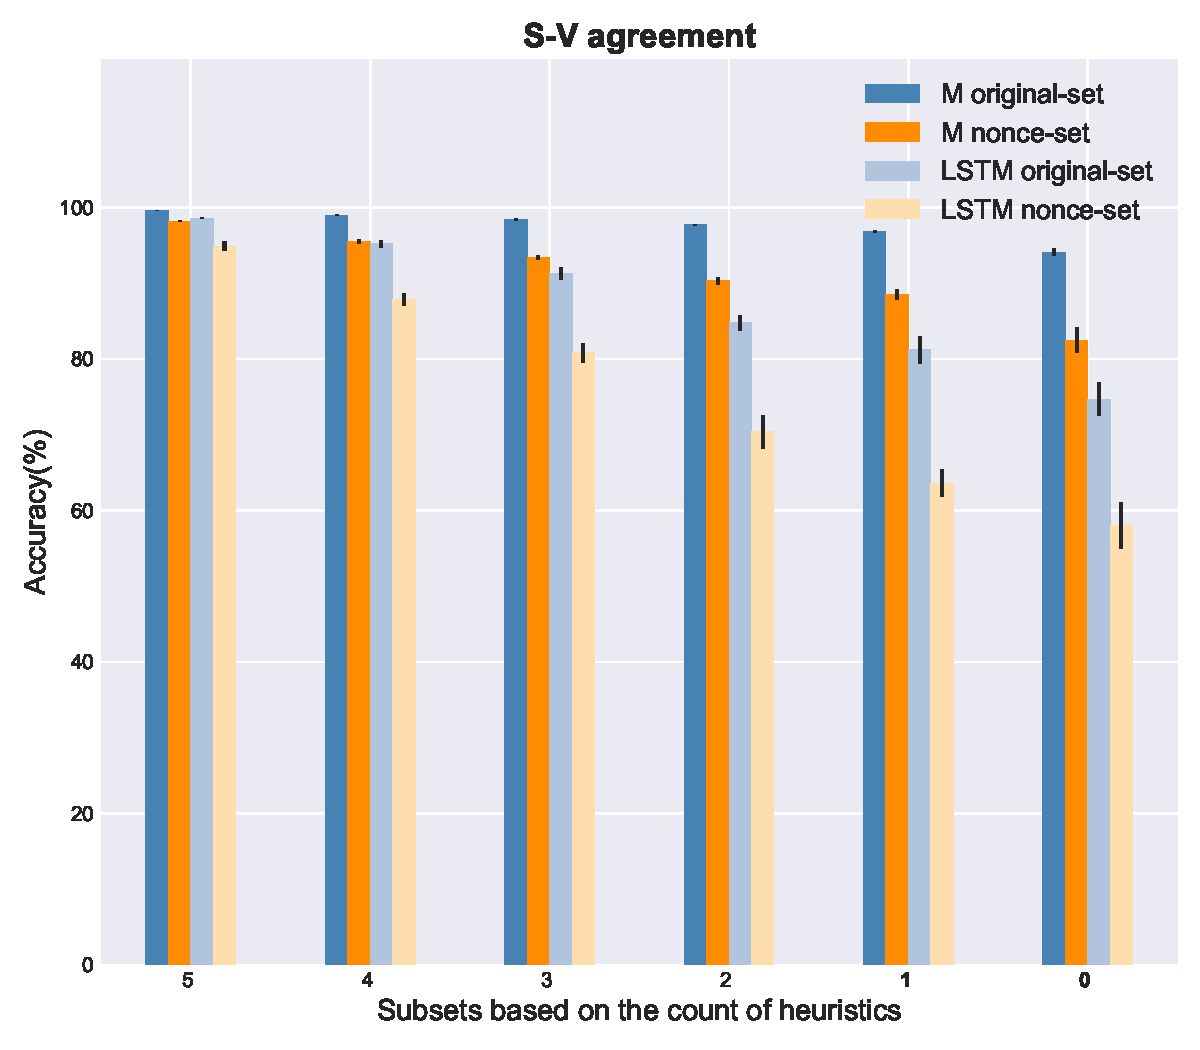
\includegraphics[width=\columnwidth]{figures/nonce_S-V.pdf}}
\scalebox{.85}{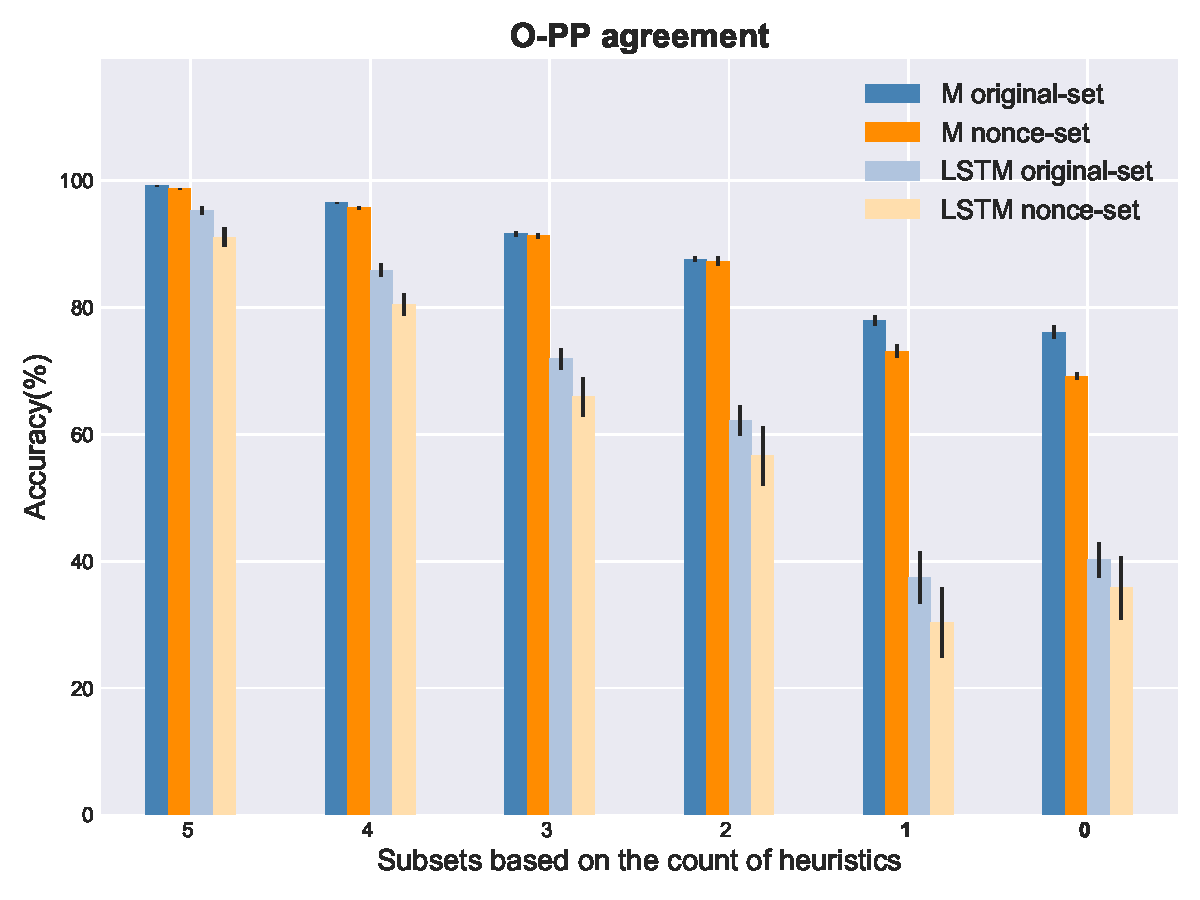
\includegraphics[width=\columnwidth]{figures/nonce_O-PP.pdf}}
\caption{Average accuracy of LSTM (indicated by lighter color bars) and Transformer models on 
 the \textit{Nonce set}, represented by orange bars, and the \textit{Original set}, indicated by blue bars.} \label{fig:nonce_heuristics}
\end{figure} 

Using the evaluation metric described in Section (\textsection\ref{sec:h_eval_protocol}), we also evaluate the syntactic abilities of the models in the \textbf{Nonce} set for the same number agreement tasks. Figure~\ref{fig:nonce_heuristics} reports models performance on the \textbf{Nonce} set compared to the original set. Overall, both architectures exhibit only a mild degradation in accuracy relative to
the \emph{original} setting across the two agreement tasks. Interestingly, the extent of performance degradation seems to correlate with the complexity of the agreement prediction task. As sentences become more abstract, semantic cues appear to have a greater impact on model decisions. Specifically, for the most challenging S-V agreement subset, the Transformer's accuracy drops by 11.6 percentage points, while the LSTM's drops by 16.7 points. For the most difficult O-PP agreement subset, 
the declines are 6.9 and 4.4 points for the Transformer and LSTM, respectively.\footnote{For detailed scores, please refer to Table~\ref{tab:nonce_heuristics} in the Appendix.} Across both agreement tasks, the observed drops in accuracy are similar in scale to what has been reported in prior studies by \cite{gulordava-etal-2018-colorless} and \cite{goldberg19assessing}, suggesting that semantic or collocational confounds have only a moderate impact on our models' performance in agreement prediction tasks.\footnote{See Section~\ref{app:lexical_freq_analysis} in the Appendix for an analysis on lexical variation in the results.}  It further implies that our models primarily rely on syntactic information to determine the correct form of the verb.


\subsubsection{Experiment 2: Impact of frequency effects} %Singular-plural asymmetry} 
\label{sec:freq_effects}

In French, as in many other languages, there is a considerable frequency disparity between singular and plural verbs. In written French, singular third-person verbs are observed to be five to ten times more common than their plural equivalents~\citep{aagren2013input}. Such frequency effects, which can influence various levels of human language processing \citep{marantz2013words}, tend to reduce errors when higher-frequency forms are the target and induce errors when a competing lower-frequency form is the target~\citep{ambridge2015ubiquity}. Empirical studies on agreement tasks involving human subjects reflect this trend. For instance, \cite{villata2017intervention} observed that French speakers tend to produce more correct agreement for the O-PP agreement when the target is singular. This trend is often attributed to human's general bias towards the production of default singular forms \citep{greenberg1963some,corbett2000gender}. These findings prompt us to investigate further: Do neural language models exhibit similar biases as humans in number agreement tasks? To what extent are the decisions made by these models a reflection of the frequency distributions encountered during training?


\begin{table}[ht]
\centering
  \begin{tabular}{l cc cc cc cc}
    \toprule 
    & \multicolumn{4}{c}{S-V} &  \multicolumn{4}{c}{O-PP}\\
    \cline{2-4}  \cline{6-8} 
    & \makecell{Singular} & \phantom{\fontsize{9}{11}\selectfont a} &
    \makecell{Plural}  & &\makecell{Singular} & \phantom{\fontsize{9}{11}\selectfont a} &
    \makecell{Plural}& \\
    \midrule  
    Transformer       & 99.4$_{\pm 0.05 }$ && 97.8$_{\pm 0.1}$ & & 99.2$_{\pm 0.1 }$ && 86.2$_{\pm 0.4}$\\
    
    LSTM        & 98.0$_{\pm 0.3}$ && 85.9$_{\pm 1.5}$ & & 95.4$_{\pm 0.7}$ && 57.2$_{\pm 2.9}$\\
    
    Argmax$_v$(target)        & 99.3$_{\pm 0.0}$ && 0.5$_{\pm 0.0}$ & & 93.2$_{\pm 0.0}$ && 8.6$_{\pm 0.0}$\\
    \bottomrule 
  \end{tabular}
\caption{Accuracy breakdown based on the grammatical number of the \target. The baseline \texttt{argmax$_v$(target)} consistently predicts the more frequently observed number of the \target. \label{tab:results_sing_plur}}
\end{table}

\begin{figure}[ht]
        \centering
        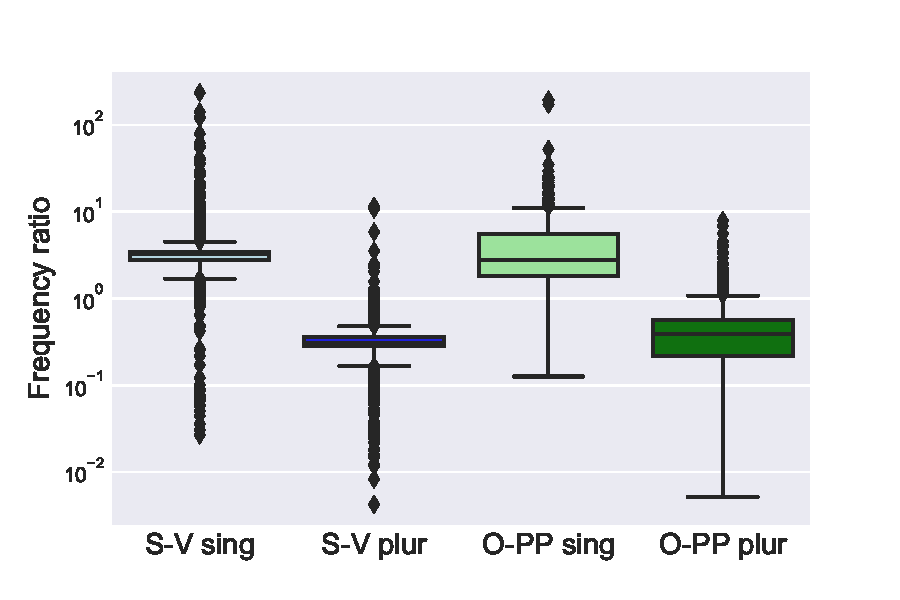
\includegraphics[width=\textwidth]{figures/rel_freq_s-v_o-pp.pdf}
        \caption{Frequency ratio of target form to competing form. For instance, for the \textit{S-V sing} condition, a ratio of $10^1$ indicates that the target verb form (singular) occurs 10 times more frequently in the pretraining data than its competing form (plural). 
        \label{fig:rel_freq}}
\end{figure}


As shown in Table~\ref{tab:results_sing_plur}, our further breakdown of the experimental results in Section~\ref{sec:heuristics} reveals consistent trends across both agreement tasks.
Transformer and LSTM achieve over 95\% accuracy in singular conditions, but show consistent lower performance in plural conditions, suggesting a model bias towards singular forms under our current evaluation metric. Additionally, this performance disparity correlates with the frequency ratio of the target form to the competing form in the pre-training data, as shown in Figure~\ref{fig:rel_freq}. This echoes the findings of \cite{ambridge2015ubiquity} that higher-frequency forms as targets tend to reduce errors. Interestingly, even though the frequency ratios for the singular class in S-V and O-PP agreements are similar, and a similar trend exists for plurals across both tasks (Figure~\ref{fig:rel_freq}), the performance gap between the plural and its corresponding singular is less pronounced in S-V agreement than in O-PP agreement (Table~\ref{tab:results_sing_plur}).


\begin{figure}[ht]
    \centering
        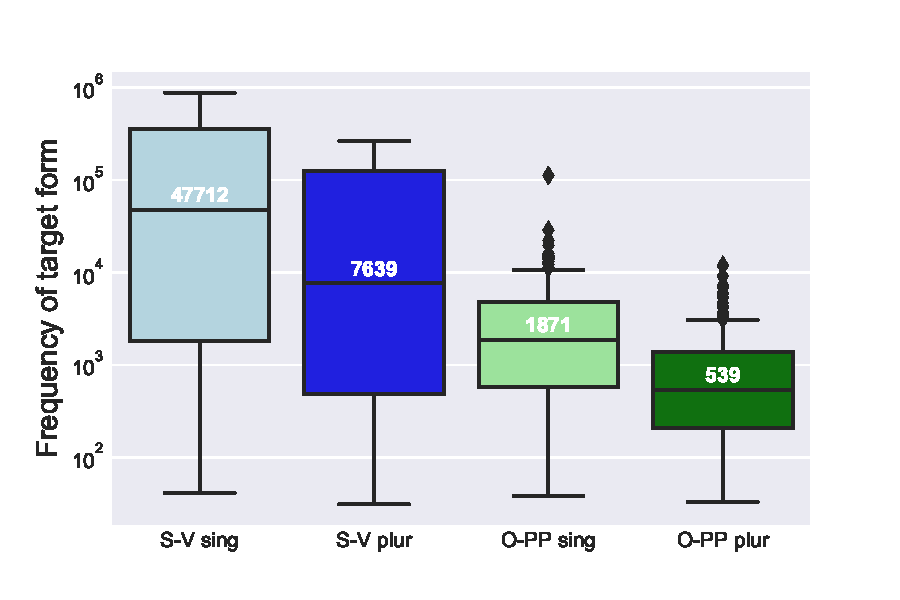
\includegraphics[width=\textwidth]{figures/abs_freq_s-v_o-pp.pdf}
        \caption{Absolute frequency of \target verbs in pre-training data, with medians displayed in white numbers}
        \label{fig:abs_freq} 
\end{figure}

In the case of S-V agreement, the Transformer model shows only a minor drop of 1.6 percentage points in accuracy for plural conditions, compared to the near-perfect accuracy with singular forms. This contrasts sharply with the near-zero accuracy of the heuristic baseline, demonstrating the Transformer's consistent preference for less frequent but grammatically correct verb forms over more frequently occurring forms. These results suggest that Transformer generally applies the subject-verb agreement rules with high accuracy, even when faced with a strong frequency bias. 

In contrast, the models' performance in O-PP agreement exhibits a significant difference between singular and plural conditions. Specifically, Transformer models experience a 13\% drop in accuracy for plural forms, while LSTMs see a more substantial decrease of over 38\%. This suggests that both types of model struggle more with plural forms in O-PP agreement compared to S-V agreement.
 Given that the O-PP agreement is a relatively rare syntactic phenomenon compared to the S-V agreement, as discussed in \S\ref{sec:h_eval_protocol}, this could partially explain the lower overall accuracy of the model in the former task. Additionally, we observe a marked discrepancy in the absolute frequency of \target verbs between S-V agreement and O-PP agreement. As depicted in Figure~\ref{fig:abs_freq}, target verbs in S-V agreement are much more frequent in models' pretraining data compared to those in O-PP agreement. For plural forms, our results align with \cite{wei-etal-2021-frequency}, indicating that more frequent target verbs are more likely to be correctly inflected in number agreement tasks. This is consistent with the frequency effects observed in human language processing. However, for singular forms, despite the absolute training frequency discrepancy of \target forms across the two agreement tasks, models show equivalently high performance on singular conditions for both tasks.  
 This suggests that, similar to humans, neural language models, may also default to using singular forms when handling number agreement tasks in French, corroborating previous research on default reasoning in language models~\citep{jumelet-etal-2019-analysing}. Notably, the Transformer model appears to be capable of effectively leveraging syntactic structures to override this default reasoning in plural conditions, as evidenced by its strong performance in both singular and plural agreement tasks.

While frequency effects could partially account for the observed asymmetry between singular and plural, task complexity also appears to play a significant role in models' lower performance in plural conditions. Further analysis of our evaluation sets reveals a consistent correlation between class distribution and task difficulty (measured by the count of heuristics; \textsection\ref{sec:h_eval_protocol}). In the easiest cases, where any of the five heuristics can solve the task (\emph{5-heuristic} subset), singular target forms predominate, accounting for 94\% of the cases in O-PP agreement and 91\% in S-V agreement. In contrast, in the most challenging cases where no heuristic allows to predict the agreement (\emph{0-heuristic} subset), the plural class becomes the dominant category (O-PP: 99\%, S-V: 96\%). This correlation holds true for both O-PP and S-V agreement. It suggests that in natural corpora, plural verbs tend to appear in more complex and potentially confounding long-distance agreement contexts compared to their singular counterparts. This further explains the models' lower performance in plural conditions. The reasons behind this empirical observation remain elusive. We intend to delve deeper into its implications in future research, using controlled experiments that account for syntactic complexity and class balance.

In summary, our analysis reveals that both Transformer and LSTM models consistently exhibit better performance in singular conditions than in plural ones across two agreement tasks. This trend suggests that these models might possess a frequency-driven bias in number agreement tasks, similar to that observed in humans. Notably, the Transformer model is better at mitigating this singular bias when processing plural conditions, highlighting its ability to leverage syntactic structures. The observed performance asymmetry could arise from several factors, including the higher frequency of singular verbs in the French language, the imbalanced distribution of grammatical number among syntactic constructions of varying complexity, and potential distinctions in how the models encode singularity and plurality, as suggested by \cite{jumelet-etal-2019-analysing}. 

\subsubsection{Experiment 3: Top-k evaluation metric} \label{sec:topK_metric}
%\paragraph{Evaluation metric} 
The evaluation metric we have adopted, which aligns with common practices in the literature  (\S\ref{chp:NA_tasks}), may introduce its own set of biases into our assessment. Specifically, our metric focuses on the model's ability to discriminate between the singular and plural forms of a target verb that naturally occur in a corpus. This approach does not necessarily capture the model's ability to generate a verb form that is both contextually appropriate and correctly inflected for number. This limitation has been noted in previous work, such as the study by \cite{newman-etal-2021-refining}, which observed that language models perform better on verbs they predict to be contextually likely. These considerations raise an important question regarding whether our evaluation metric faithfully reflects the models' likely behavior. In other words, do the most likely words, predicted by the models given a sentence prefix, exhibit consistent agreement features as those obtained from our \textit{target verb} evaluation metric?



To address this question, we propose an alternative evaluation metric, referred to as the $top$-3 evaluation metric, to better measure models likely behavior. Instead of comparing the probabilities of two forms given an evaluation sentence prefix, we focus on the words the models consider most likely to occur. Specifically, we sample the top ten most probable word predictions made by the models for a given sentence prefix. From these words, we use the morphologizer of a pre-trained French model in \textit{spaCy}~\citep{spacy},\footnote{\url{https://spacy.io/models/fr}, we used the model: \textit{fr\_dep\_news\_trf}} to get the three most probable verbs. We then consider the majority number expressed among these three verbs as the models' agreement prediction for that sentence. To ensure a fair comparison between our initial evaluation metric and this $top$-3 evaluation metric, we exclude sentences where the top ten most probable word predictions from the models do not contain any verbs.\footnote{For the Transformer model, we excluded 7.9\% (resp. 29.8\% for LSTM) of the total evaluation sentences (27,582) in the S-V agreement. Similarly, in the O-PP agreement task,  0.3\% of the total evaluation sentences (68,497) were excluded for the Transformer, compared to 45.7\% for the LSTM. Among the excluded sentences, the top ten LSTM predictions are mainly punctuation, prepositions, articles, or nouns. }
 % (resp. LSTM)
\begin{figure}[ht]
    \centering
    \begin{subfigure}[b]{0.49\textwidth}
        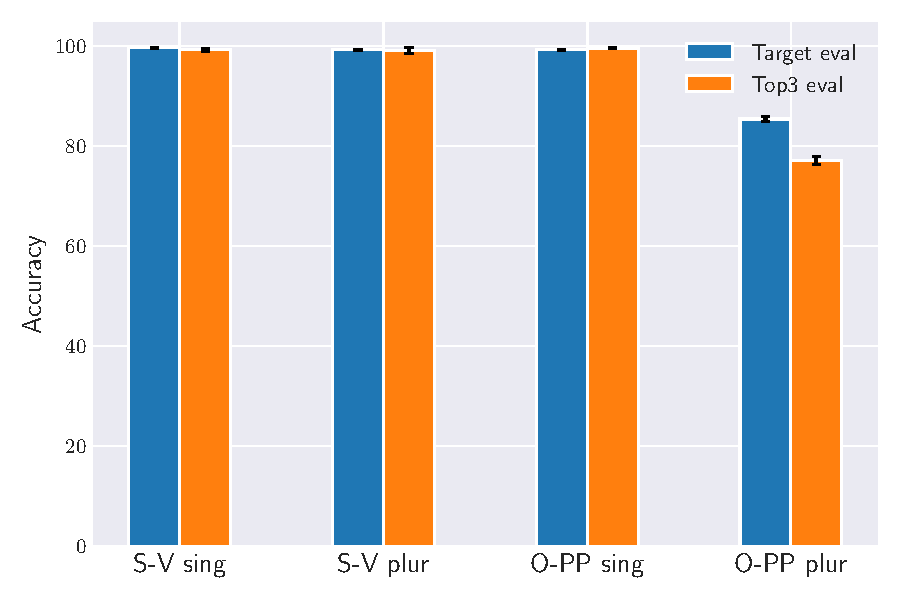
\includegraphics[width=\textwidth]{figures/tm_2_eval.pdf}
        \caption{ \textbf{Transformer} language model}
        \label{fig:tm_2_eval}
    \end{subfigure}
    \hfill
    \begin{subfigure}[b]{0.49\textwidth}
        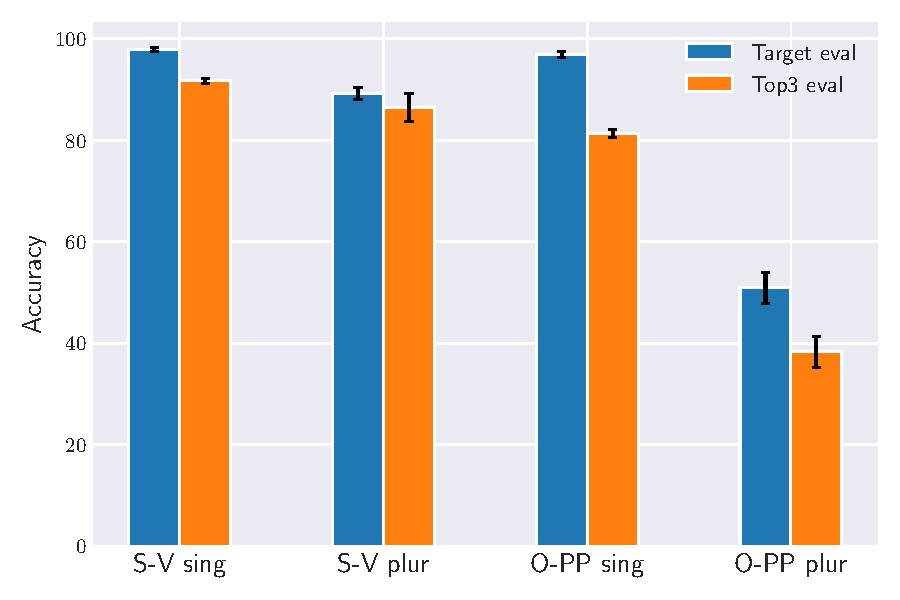
\includegraphics[width=\textwidth]{figures/lstm_2_eval.pdf}
        \caption{ \textbf{LSTM} language model
        }
        \label{fig:lstm_2_eval}
    \end{subfigure}
    \caption{Comparison of models' accuracy in two agreement tasks using $top$-3 evaluation metric (orange bars) and \textit{target verb} evaluation metric (blue bars).}
\end{figure}


As shown in Figures~\ref{fig:tm_2_eval} and~\ref{fig:lstm_2_eval}, the trends observed with the $top$-3 evaluation metric closely align with those of the \textit{target verb} evaluation metric. For both Transformer and LSTM, the two metrics demonstrate a persistent performance asymmetry between singular and plural conditions in both agreement tasks. The performance breakdown based on task difficulty (Table~\ref{tab:tm_full_2_eval} and \ref{tab:lstm_full_2_eval} in the Appendix) also indicates that all models performance decrease with the task difficulty. Notably, for the Transformer, a high level of consistency is observed between the two metrics, with an inter-agreement rate surpassing 92\% in both tasks (see Table~\ref{tab:inter_agreement} in the Appendix for full results).

For the Transformer model, the two evaluation metrics yield similar scores for the S-V agreement and the singular condition of O-PP agreement. However, a decrease of 8.3\% is observed in the plural condition of the O-PP agreement when using the $top$-3 metric. This decrease may be partially attributed to the presence of part-of-speech ambiguous words (e.g., ``données" can be both a noun and a verb) or number ambiguous words (e.g., ``appris" can be both a singular and plural form). In contrast, the strong baseline model, LSTM, consistently exhibits lower accuracy across the board when evaluated with the $top$-3 metric. Additionally, for both agreement tasks, over 29\% of the top ten predictions of LSTM (compared to less than 8\% for Transformers) do not contain any verbs. This finding indicates that the Transformer model demonstrates similar behavior under the two evaluation metrics and exhibits more robust syntactic behavior compared to the baseline LSTM model.

Given the similar performance trends of the Transformer on both agreement tasks across two evaluation metrics, we consider the differences between these metrics minor enough to proceed with the main objective of our study: investigating how the Transformer LM represents syntactic structures when handling two superficially similar long-distance agreement phenomena. Additionally, we want to avoid the potential noise introduced by the $top$-3 evaluation metric, which relies on a pre-trained model to predict morphological features. 
Therefore, all subsequent experiments are conducted using the \emph{target verb} evaluation metric, aligning with the common practice in the literature (\S\ref{chp:NA_tasks}).


Interestingly, our findings based on naturalistic corpora diverge from the observations of \cite{newman-etal-2021-refining}. While their study, using synthetic data, suggests that models perform better on verbs predicted to be the most likely in context, we did not observe this improvement in our study. Future research could further investigate the contributing factors to the observed performance asymmetry between singular and plural forms. This could involve artificially manipulating the relative frequency of singular and plural nouns within different constructions in the model's training data to better understand their influence on performance.


\subsection{Conclusion}
In this section, we evaluated the autoregressive Transformer's ability to process two syntax-sensitive phenomena in French, using number agreement tasks. Our initial experiments demonstrate strong overall performance for both types of agreement, indicating that the model's behavior aligns closely with human language use. Furthermore, we investigated the impact of surface heuristics and other known confounding factors on the model's performance. These findings lend further support to existing research (Section \ref{sec:review_structure_nlm}), confirming that the Transformer model exhibits a robust capability to capture and generalize syntactic information beyond surface heuristics and semantic or collocational cues. 

We observed that while the Transformer does show some sensitivity to frequency effects, it generally displays a consistent preference for grammatically correct forms, effectively overcoming strong biases present in the training data. Compared to the LSTM, a strong baseline in the literature for evaluating syntactic abilities of NLMs (\S\ref{chp:NA_tasks}), the Transformer is less influenced by surface heuristics and frequency effects, and exhibits more consistent performance under different evaluation metrics. These findings suggest that the Transformer meets the first criterion --- behavioral-level similarity --- for genuine syntactic generalization.

Additionally, it is important to recognize that humans also make agreement errors~\citep{BOCK199145}, and also display a bias favoring singular forms, leading to fewer agreement errors for these forms in French object-past participle agreement tasks, as observed by ~\cite{villata2017intervention}. In this context, the heuristics that affect the model's performance might hold relevance not just for the domain of artificial neural networks, but could also offer valuable insights into the study of human linguistic abilities. Specifically, these heuristics could stimulate the development of testable hypotheses for experiments aimed at understanding human syntactic performance. Our heuristic-based approach for crafting evaluation sets could help to build stimuli that effectively measure human capacity for rule-based linguistic generalization.


\section{Locating syntactic information in Transformer language model} \label{sec:probing_location}

The experiments presented in the previous section demonstrate that the Transformer language model consistently outperforms the strong baseline model, LSTM, in long-range subject-verb and object-past participle agreements. Crucially, Transformer is able to abstract away from potential confounds such as lexical co-occurrences or superficial heuristics. This successful behavioral assessment allows us to delve deeper to evaluate the Transformer's representational adequacy as a model that helps to explain human syntactic processing.
In light of this success, which aligns with prior research indicating that Transformers capture a “substantial amount” of syntactic information (\S\ref{sec:review_structure_nlm}), two questions emerge naturally: First, where is this syntactic information located within the Transformer's internal representations? Second, given the superficial similarities between the two types of agreement tasks we studied, does the Transformer model use a uniform internal representation for both, or are there distinct representations that reflect the theoretical nuances of each task?


In this section, focusing on Transformer LM, we investigate the question of \textbf{where} syntactic information is encoded from two perspectives.\footnote{Datasets and code: \url{https://gitlab.huma-num.fr/bli/syntactic-info-distribution}} First, in Section~\ref{sec:within_sentences}, we use probing classifiers, detailed earlier in Section~\ref{sec:probing}, to identify token positions where the agreement information is encoded within the model's internal representation. 
This analysis enables us to localize the agreement feature across token representations within a sentence. Second, in Section~\ref{sec:within_repr}, we use a feature selection method associated with probing to identify the specific subspace within the Transformer's representations that encodes the relevant agreement information.
 

\subsection{Distribution of syntactic agreement information across token positions}\label{sec:within_sentences}
In this section, we investigate where the Transformer encodes the syntactic information necessary for predicting the correct \emph{target} form in the two types of agreement tasks. Specifically, we explore whether this agreement information is distributed across all tokens following the \emph{cue} in the sentence, as theoretically allowed by the self-attention mechanism and observed by \cite{klafka-ettinger-2020-spying}. Alternatively, is this information encoded more locally, centered around the \cue and \target tokens, as predicted by the specific agreement rules?

To investigate these hypotheses, we use probing classifiers following the approach of \cite{giulianelli-etal-2018-hood} (\S\ref{chp:NA_tasks}). In our study, 
 we denote the representation generated by a Transformer LM for the token $t$ at layer $l$ by:
 \begin{equation}
 r_t = \text{Transformer}_l(t) 
 \end{equation}
 Given an evaluation sentence, our goal is to examine whether the representation of a token $t$ within the sentence contains the relevant syntactic agreement feature, denoted as $\mathcal{A}$, which corresponds to the number of the \cue (either `Singular' or `Plural'). To achieve this, we train a classifier defined as a function $\mathcal{C}$ that maps the representation of each token to the agreement feature of the sentence, $\mathcal{A}$:
\begin{equation}
\mathcal{C}:r_t \leadsto \mathcal{A}, \text{with } \mathcal{A} \in \{\text{Singular}, \text{Plural}\}
\end{equation}



The core assumption underlying this approach is that if the Transformer has encoded syntactic agreement information within its representation space, then a probing classifier should be able to ``extract'' this information from the corresponding token representations produced by the Transformer (\S\ref{sec:probing}). 
In this study, we use a logistic regression classifier,\footnote{This choice follows the recommendation of ~\cite{hewitt-liang-2019-designing}, who found that non-linear probes tend to memorize the probing task by leveraging surface pattern recognition, rather than relying on the information captured in the representations of the probed model.} defined as:
\begin{equation}
 \sigma(\theta^T r_t + b) \leadsto \mathcal{A}, \text{with } r_t \in \mathbb{R}^{768} 
\end{equation}
Here, $r_t$ is the token representation extracted from the Transformer's last layer (i.e., the 16th layer in our experiments) for the token $t$, $\sigma$ denoting the sigmoid function. The parameters vector (i.e., coefficients) is represented by $\theta$, and $b$ represents the bias term. 

 \begin{figure}[htbp]
  \centering
  \pgfsetlayers{depgroups,main}
 \scalebox{0.86}{\begin{dependency}
    \tikzstyle{POS}=[font=\fontsize{10}{12}\selectfont]
    %\tikzset{POS/.style={font=\fontsize{9}{11}\selectfont}}
    \depstyle{pref}{draw=blue, fill=blue!25}
    \depstyle{cont}{draw=yellow, fill=yellow!25}
    \depstyle{suf}{draw=green, fill=green!25}
    
    \begin{deptext}
    Sans \& doute \& ces \& {\bf moments}\& de \& \underline{bonheur} \&  que \& son \& \underline{frère} \& lui \& a \& {\bf donnés}  \_\_ \& \  {\bf resteront} \& ... \\
        |[POS]| No \& |[POS]| doubt \& |[POS]| these \& |[POS]| moments\_Pl \& |[POS]| of \& |[POS]| happiness\_Sg \& |[POS]| that \& |[POS]| his \& |[POS]| brother\_Sg \& |[POS]| (to) him \& |[POS]| has  \& |[POS]| given\_Pl \& |[POS]| will\_stay\_Pl \& ...\\ 
     \&  \&  \& {\bf cue} \&  \&  \&  \& \&  \& \& \& {\bf target}  \&  \&  \\
    \end{deptext}
    \depedge[edge unit distance=1ex]{7}{4}{antecedent}
    \depedge[edge unit distance=.5ex]{12}{7}{object}
    %\depedge[edge unit distance=1ex]{13}{4}{nsubj}
    \wordgroup[pref]{1}{1}{2}{prefix}
    \wordgroup[cont]{1}{3}{11}{context}
    \wordgroup[suf]{1}{13}{14}{suffix}
  \end{dependency}}
  \caption{ For the O-PP agreement, the prefix is highlighted in blue, the context in yellow and the suffix in green.
  \label{fig:probing_zones}}
\end{figure}

% \textcolor{blue}{\bf target-v}

\paragraph{Training} To train the probing classifiers, we construct a training set $\mathcal{D} = \{x^{(i)}, \mathcal{A}^{(i)}\}$ as follows. For each token in the sentences of our evaluation set, we extract its representations from the last layer of the Transformer and associate it with a label $\mathcal{A}^{(i)} \in \{ \textrm{Singular}, \textrm{Plural} \}$ indicating the number of the \cue. Next, as illustrated in Figure~\ref{fig:probing_zones}, we divide each sentence into three parts: 
\begin{itemize}[topsep=0pt,itemsep=-1ex,partopsep=1ex,parsep=1ex]
    \item \emph{prefix}: words before the \cue and its dependent words;
    \item \emph{context}: words from the \cue (and its dependent words) to just before the \target;
    \item \emph{suffix}: words following the \target
\end{itemize}
\noindent We train individual probing classifiers for each category of word within each part of the sentences. This approach allows each classifier to specialize in PoS-specific representations of long-distance agreement information. To ensure fair comparison across sentence parts, we exclude tokens with PoS tags that occur less than 100 times, namely SYM, SCONJ, INTJ, PART, and X. This results in a total of 11 token categories in each sentence part, giving us $11*3$ probing classifiers.

For training and evaluation, we split the examples into 80\% training data and 20\% evaluation data. Each classifier is trained using three different train/test splits.\footnote{All classifiers were implemented with the \texttt{scikit-Learn} library~\cite{scikit-learn}. A grid search with 5-fold cross-validation was performed to select the optimal value of the regularization parameter $C$. The \texttt{max\_iter} parameter was set to 1,000 during the training process. Random\_state = 0, 20 and 42} The averaged results are reported in Table~\ref{res:probing_high_level}, and more detailed results per word category are provided in Figure~\ref{tab:res_per_PoS} of the Appendix.

\begin{table}[ht]
    \centering
  \begin{tabular}{l cc cc c}
    \toprule 
    & \multicolumn{4}{c}{Mean probing Accuracy } \\
    \cline{2-5}
    & \makecell{O-PP agreement \\ } & \phantom{\fontsize{9}{11}\selectfont a} &
    \makecell{S-V agreement} & \phantom{\fontsize{9}{11}\selectfont a}  \\
    \cline{2-2} \cline{4-4} 
    \emph{prefix}        & 58.6\%$_{\pm 0.1}$ && 59.5\%$_{\pm 0.2}$ &\\
    \emph{context}       & 92.3\%$_{\pm 0.2}$ && 93.0\%$_{\pm 0.1}$ \\
    \emph{suffix}       & 73.6\%$_{\pm 0.2}$ && 78.1\%$_{\pm 0.2}$  \\
    \bottomrule 
  \end{tabular}
\caption{Probing results across different sentence parts (see
  Figure \ref{fig:ex_agreement}). The reported scores represent the average accuracy of all PoS-based classifiers for each sentence segment. \label{res:probing_high_level}}
\end{table}

\paragraph{Results} The average accuracy achieved by our probes on different parts of the sentence is presented in Table~\ref{res:probing_high_level}. We observe a similar pattern for both O-PP and S-V agreement: the syntactic agreement information about the number of the \cue is essentially encoded within the tokens of the \emph{context}. It is not distributed across all tokens following the cue in the sentence.

As expected, in both tasks, the probe performance on the \emph{prefix} is very low. Given the autoregressive nature of the model, token representations in the \emph{prefix} cannot attend to the \cue, and thus, cannot encode its number information. The accuracy observed on the \emph{prefix} mainly reflects the difference in prior probabilities of the two grammatical number classes within the evaluation set.\footnote{As discussed in \S\ref{sec:NA_data}, within the two evaluation sets, 65\% of the target past participles in O-PP agreement are singular, while 70\% of the target verbs in S-V agreement are singular.} In contrast, when using tokens from the \emph{context} as input features, the probe accuracy is consistently high for both agreement types. However, the accuracy significantly drops for the \emph{suffix} tokens, though it remains higher than that observed for the \emph{prefix}. This suggests that the information required to predict the correct \emph{target} form is distributed across all tokens between the \emph{cue} (where the number of the \emph{target} verb is specified) and the \emph{target} (where this information is being `used'). This finding, to some extent, challenges the observations of \cite{wisniewski-etal-2021-screening}, who discovered that gender information in a neural translation system is distributed throughout the source and target representations. However, it should be noted that their study focused on a different type of information and was limited to sentences with a simple structure.

 
Results so-far indicate that the agreement information related to \cue is mainly distributed across all tokens in the \emph{context} part of the sentences. To gain a more precise understanding of how the Transformer model tracks this agreement information from \cue to \target, we conduct an experiment that focused on a specific sentence pattern with a fixed six-word \emph{context}. Specifically, we focus on sentences where \cue is
separated from the relative pronoun only by a prepositional
phrase. This pattern applies to sentences such as the one shown in (\ref{ex:S_V_fixed_probing}) for long-distance subject-verb agreement, and (\ref{ex:O_PP_fixed_probing}) for object-past participle agreement.

\begin{exe}
    \ex \label{ex:S_V_fixed_probing}
    \begin{tabular}{lllllllll}
    Sentence: & ... & \textbf{bureau·x} & en & métal & qu' & il & aime & \textbf{coût·ent } ... \\
    & ... & {\scriptsize desks} & {\scriptsize Prep.} & {\scriptsize metal} & {\scriptsize that} & {\scriptsize he} & {\scriptsize loves} & {\scriptsize cost }... \\
    Pattern: & ... & \texttt{Subject} & \texttt{ADP} & \texttt{NOUN} & \texttt{que} & \texttt{PRON} & \texttt{V} & \texttt{target V}...
    \end{tabular}
\end{exe}

\begin{exe}
\ex \label{ex:O_PP_fixed_probing}
\begin{tabular}{lllllllll}
   Sentence: & ... & \textbf{bureau·x} & en & métal & qu' & il & a & \textbf{trouvé·s } ... \\
   & ... & {\scriptsize desks} & {\scriptsize Prep.} & {\scriptsize metal} & {\scriptsize that} & {\scriptsize he} & {\scriptsize has} & {\scriptsize found\_Pl } ... \\
   Pattern: & ... & \texttt{Antecedent} & \texttt{ADP} & \texttt{NOUN} & \texttt{que} & \texttt{PRON} & \texttt{AUX} & \texttt{target PP }...
\end{tabular}
\end{exe}

\paragraph{Training} To examine the distribution of the agreement information between the \emph{cue} and the \emph{target}, we build a dataset for each agreement phenomenon, following the previously defined patterns with a fixed six-word \emph{context}. Each position within the \emph{context} is labeled with the corresponding PoS tag of the tokens, as illustrated in (\ref{ex:S_V_fixed_probing}) and (\ref{ex:O_PP_fixed_probing}). Additionally, we also consider the five tokens before and after the six-word \emph{context} window, denoted as \texttt{$b_i$} (for tokens before) and \texttt{$a_i$} (for tokens after), where \texttt{i} represents the position relative to the pattern, as illustrated by the X-axis labels in Figure~\ref{fig:fix5}.


For the training set, we randomly sample 800 examples for each agreement phenomenon, ensuring a balance between singular and plural forms. For the test set, we sample a balanced set of 200
examples, with 100 sentences where the embedded noun (at the `NOUN' position within the \emph{context}) is an \emph{attractor}, and 100 sentences where this noun has the same number as the \emph{cue}.\footnote{We conducted the sampling process using three different seeds, and for each sampling, we performed three train/test splits. The reported scores are averaged across all splits.} Unlike the previous experiment where we trained probing classifiers on representations of all words in the sentence based on their word categories and their location in the sentence, in this experiment, we train distinct classifiers for each position within the defined scope of sentences.
%, as illustrated by the x-axis labels in Figure~\ref{fig:fix5}.

\begin{figure}[htbp]
    \begin{subfigure}{\textwidth}
        \centering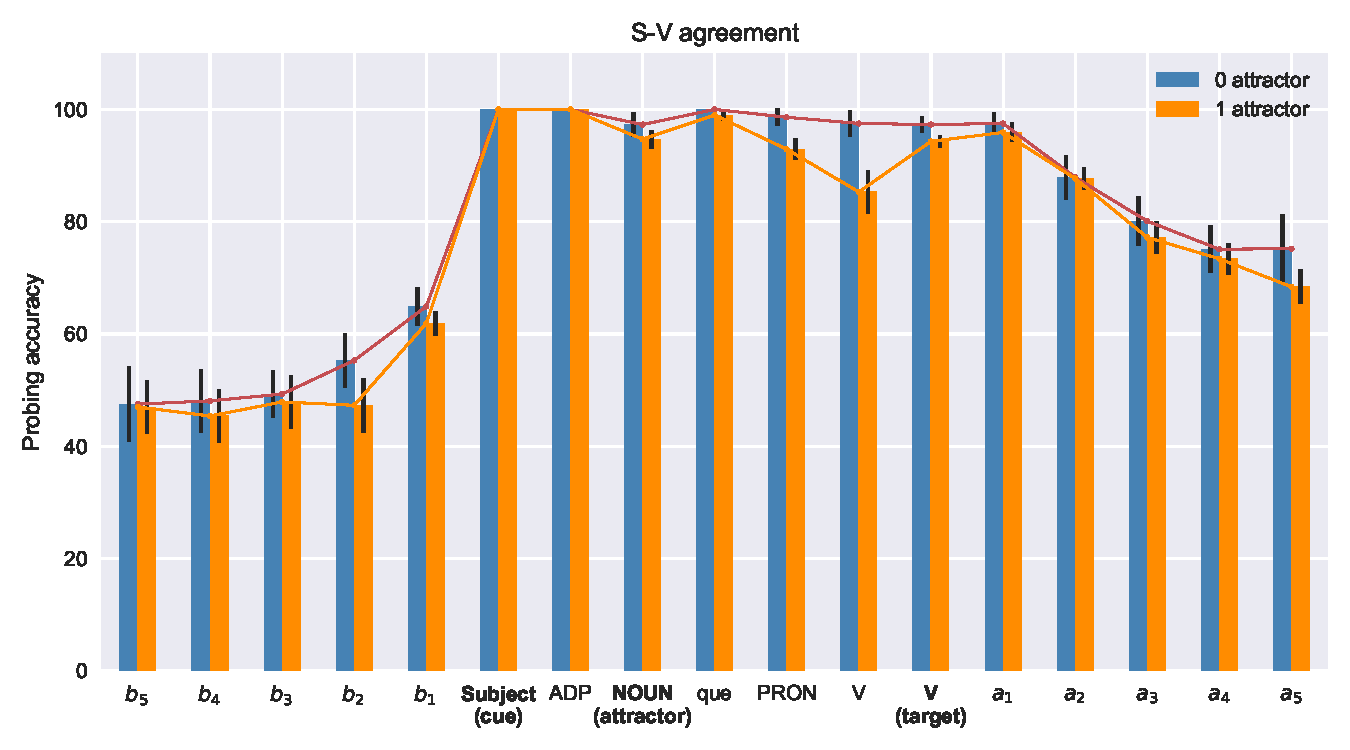
\includegraphics[width=0.95\textwidth]{figures/probing_subj-v.pdf}
    \end{subfigure}
    \vspace{0.2cm}
    \begin{subfigure}{\textwidth}
        \centering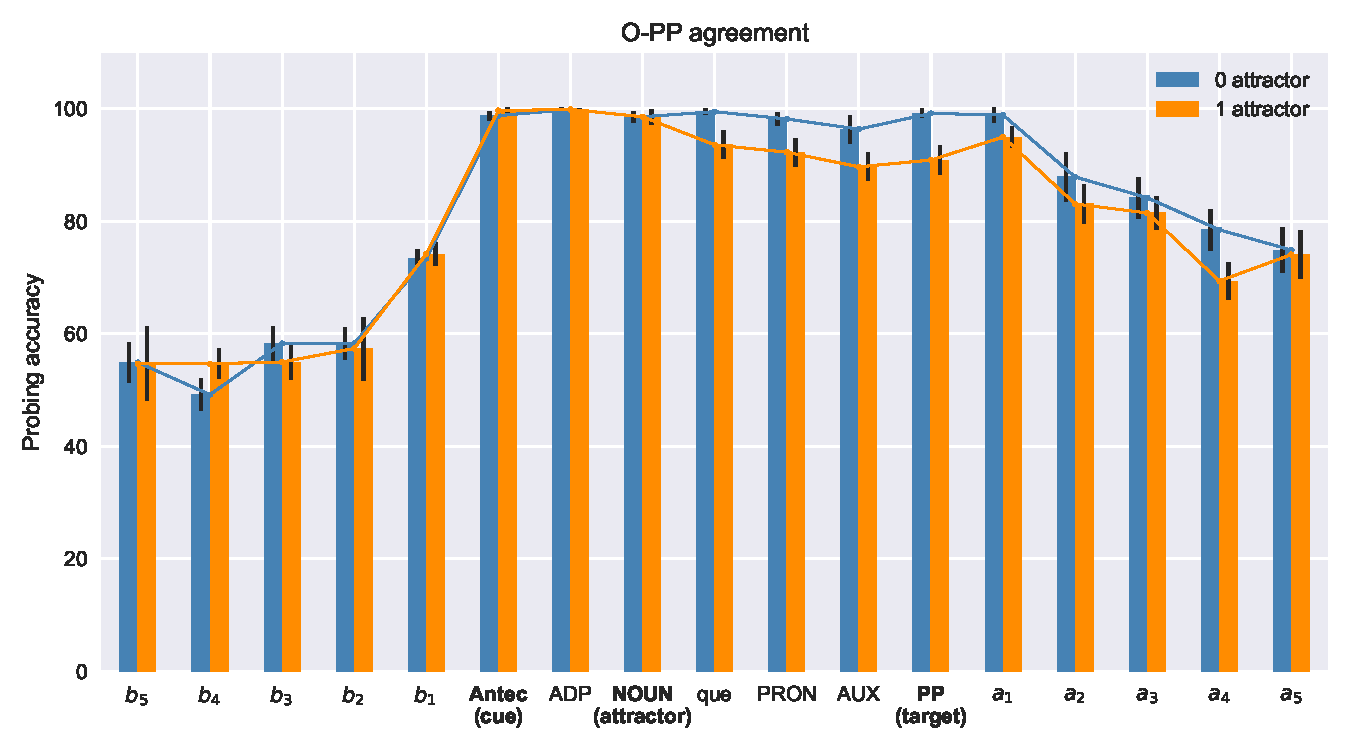
\includegraphics[width=0.95\textwidth]{figures/probing_obj-pp.pdf}
    \end{subfigure}
    \caption{Average probing accuracy at each position based on the number of the
      \emph{cue}. The \texttt{b$_i$} (resp. \texttt{a$_i$}) position
      denotes the $i$-th token before (resp. after) the pattern. The position labeled as `Noun' corresponds to a noun with the opposite number as the \emph{cue} in the 1-attractor subset, and a noun with the same number as the \emph{cue} in the 0-attractor subset.
      \label{fig:fix5}}
\end{figure}

\paragraph{Results} 
We plot in Figure~\ref{fig:fix5} the average probing accuracy at different positions of the specific construction for both agreement phenomena. The results show a consistent pattern: the accuracy of the probes is initially low in the \emph{prefix} (i.e., b-positions) but starts to increase from the position just before the \emph{cue}. This position often corresponds to determiners or adjectives that need to agree in number with the \emph{cue}. As we move into the \emph{context}, the accuracy stabilizes, with probes achieving very high accuracy, even at the attractor position. The accuracy then drops sharply after passing the \emph{target}, especially when an attractor is present in the \emph{context}. It appears that once the \emph{target} has been encountered and the number information of the \emph{cue} is no longer relevant, subsequent tokens no longer encode it. This trend is consistently observed for both types of agreement phenomena. 

Unsurprisingly, the probes achieve perfect scores at and just after the \emph{cue} positions, as well as at the position immediately following the \emph{target}. This suggests that the Transformer has learned to recognize and store the number information of the \emph{cue} and \emph{target} in its internal representations. And this information is encoded in a linearly extractable manner.  

A particularly interesting observation arises when considering the \textit{1-attractor} subset. The accuracy of the probes only slightly degrades at positions immediately following the attractor, which carries the opposite number to the probed grammatical number. Intriguingly, at the target position, where the agreement information from the \emph{cue} is being used, the probe accuracy shows a reboost, in particular in S-V agreement. This suggests that the model appears to know where to pinpoint the syntactic number information, enabling it to avoid potential misleading cues. These observations suggest a coherent and robust flow of agreement information within the Transformer's representations. 


\subsection{Probing internal representations components} \label{sec:within_repr} 
Our previous experiment using probing classifiers revealed that agreement
information is encoded across all tokens within the \emph{context}. In this study, we aim to determine \textbf{where} within the Transformer's representation space this information is encoded. Specifically, we want to identify which components of the token representations generated by the Transformer are most crucial for capturing this syntactic agreement information.

To achieve this, we use an $\ell_1$-regularized logistic regression model,
known for its tendency to produce sparse feature vectors by driving many feature coefficients, denoted by $w_i$ in the equation (\ref{eq:LR_weights}), towards zero \citep{tibshirani96regression,ng2004feature}. This characteristic makes it well-suited for feature selection tasks, allowing us to identify the most relevant components within the Transformer's representations that are responsible for capturing the agreement information.
The $\ell_1$-regularized logistic regression model follows the formulation:
\begin{equation}
\begin{aligned}
\mathbb{P}_{\ivec{w},b}(y=\text{Singular}|x_i) &= \sigma(\ivec{w}^T x_i + b),  \\
\text{where } \ivec{w}^T x_i &= w_1*x_1 + w_2*x_2 + \ldots + w_{768}*x_{768}
\end{aligned}
\label{eq:LR_weights}
\end{equation}
where $\ivec{w}$ represents the parameter (i.e., coefficients) vector, $x_i$ denotes the token representation at position $i$ in a sentence, and $y$ represents the grammatical number of the \cue, which is the agreement information. This model minimizes the objective function with an $\ell_1$ regularization term:
\begin{equation}
    \sum_{i=1}^n -\log P(y_i | \ivec{x}_i;\ivec{w}) + \frac{1}{C}||\ivec{w}||_1
\end{equation}
where, $C$ represents the inverse of regularization strength. As the value of $C$ increases, the number of features with non-zero coefficients $w_i$ also increases. By varying the values of $C$, we can control the sparsity level of the solution $\ivec{w}$, thereby identifying the most relevant components of the Transformer's representations for the probing tasks. 

\begin{figure}[htbp]
  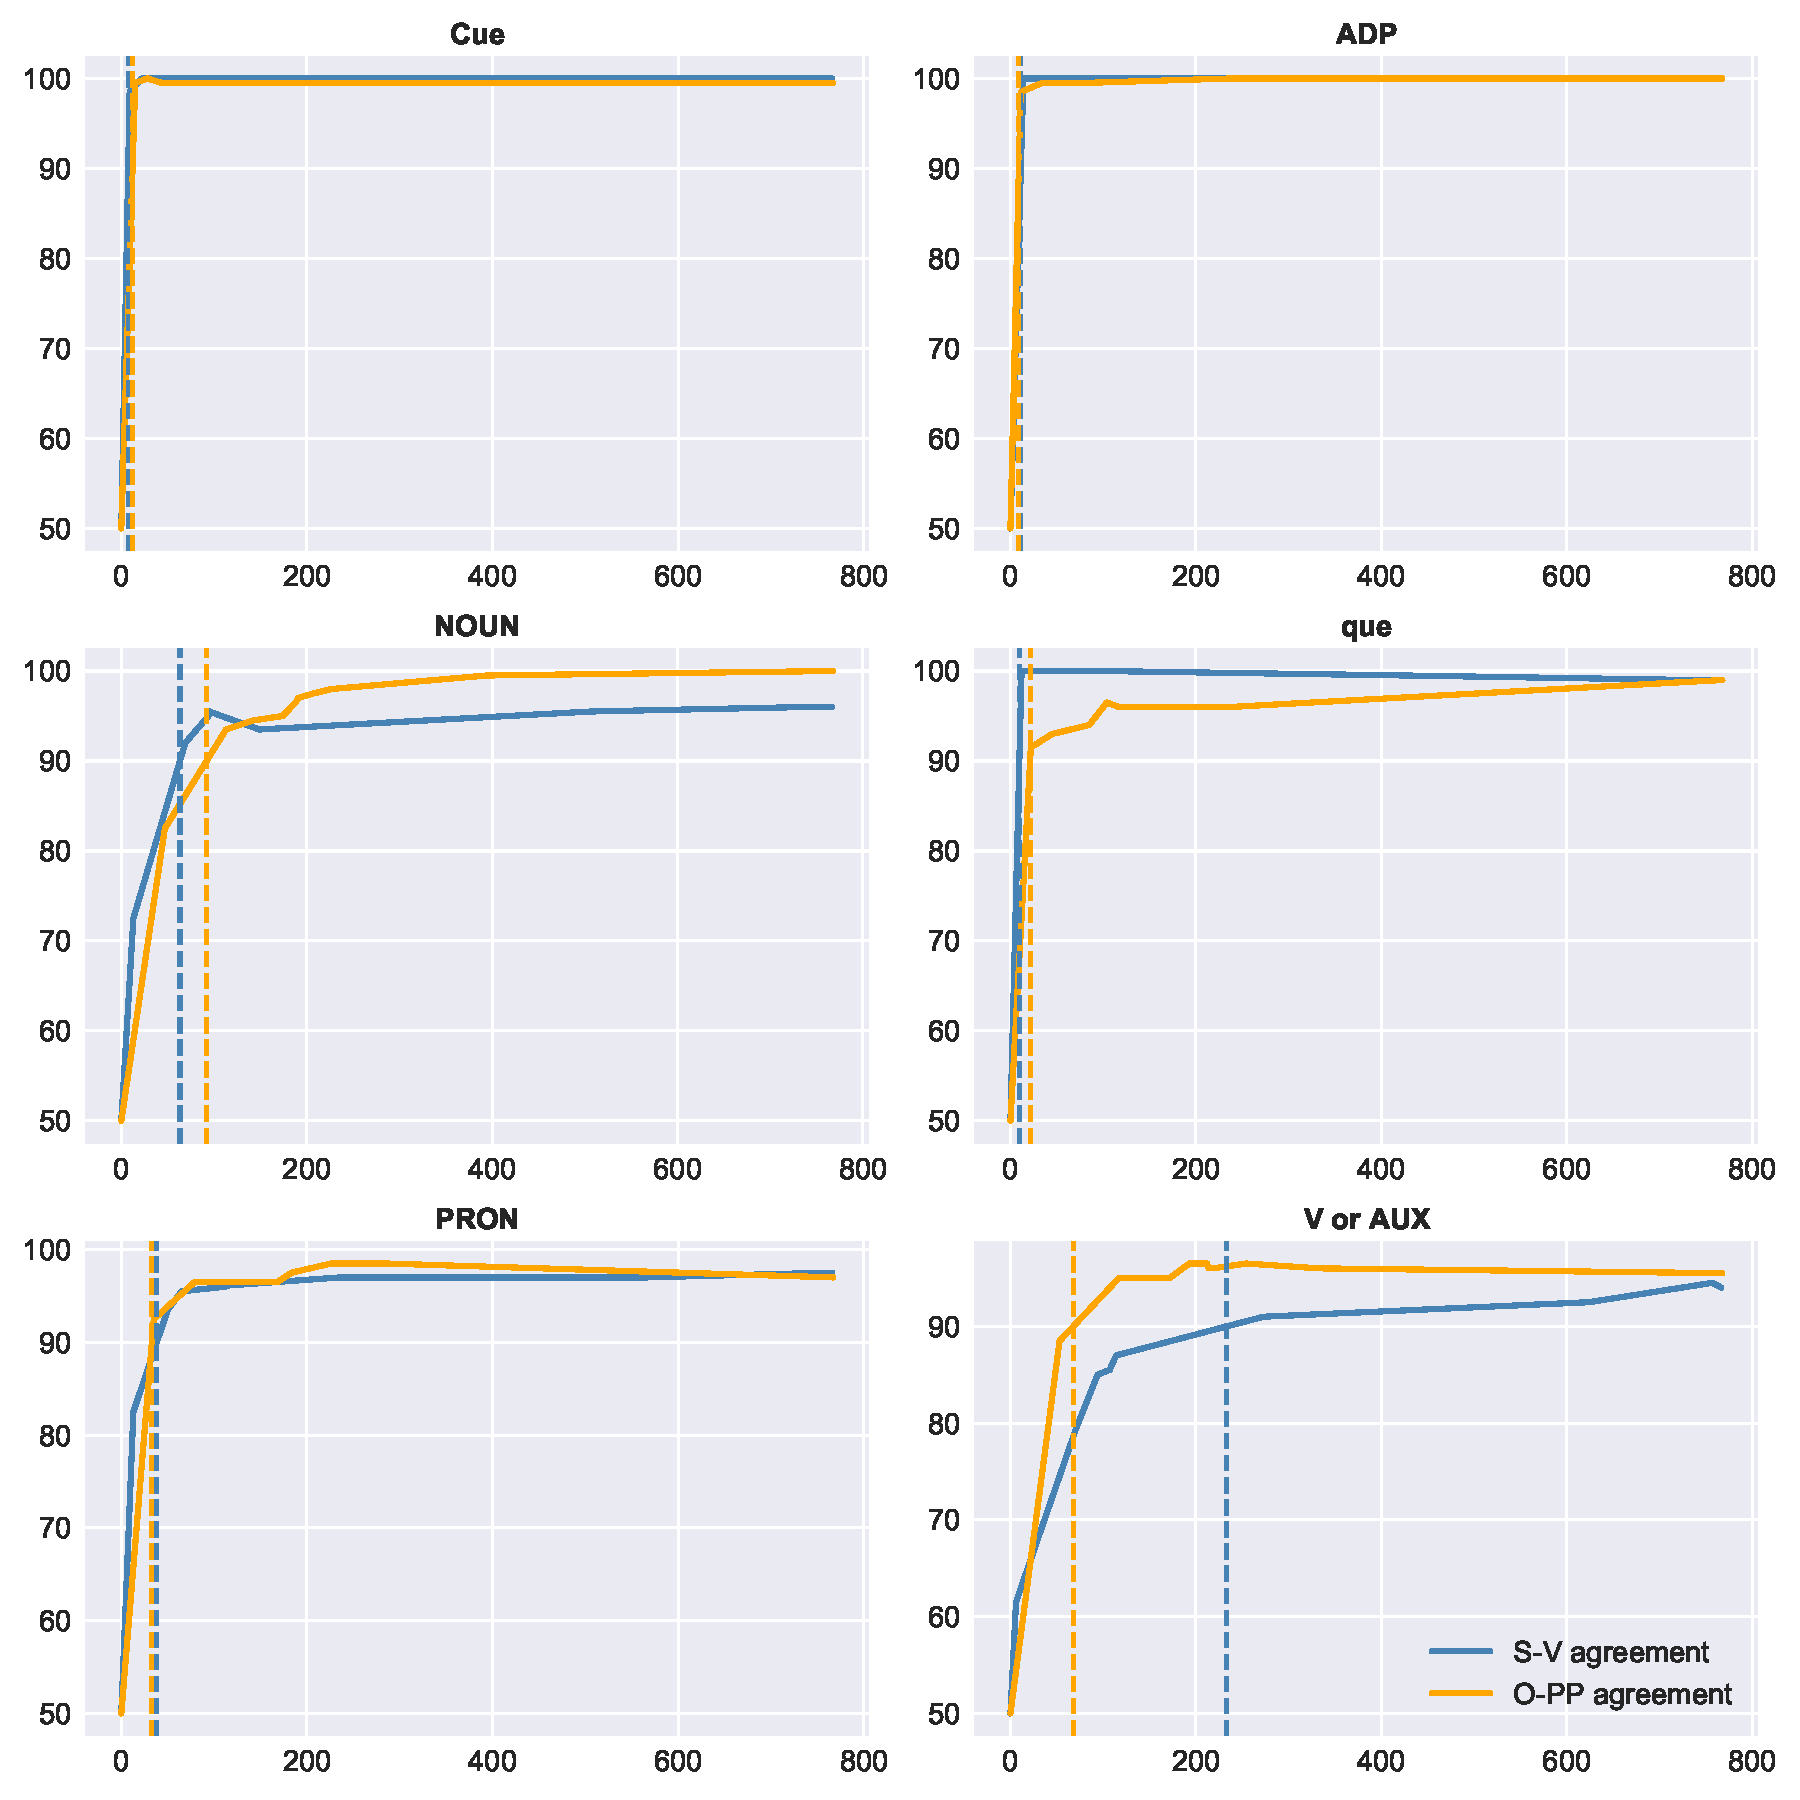
\includegraphics[width=\columnwidth]{figures/probing_c-path.pdf}
  \caption{Probing accuracy as a function of the count of dimensions (for 768-dimension token representations)  with non-zero coefficients, obtained through feature selection using $\ell_1$ regularized logistic regression for each position within \emph{context}.
  The X-axis denotes the count of non-zero coefficient dimensions, and the Y-axis represents probing accuracy. Vertical dashed lines indicate the points at which the accuracy reaches 90\%. 
    \label{fig:res_C_path}}
\end{figure}

\paragraph{Training} In contrast to the previous experiment where we assessed probing accuracy with a fixed optimal regularization parameter $C$, in this study we vary the values of $C$ in the $\ell_1$-regularized logistic model as a means for feature selection. We replicate the same task from Section~\ref{sec:within_sentences}: training a classifier to map token representations to a binary label indicating the grammatical number of the \cue. We use the same training and evaluation dataset: sentences of six-word \emph{context} (\S\ref{sec:within_sentences}). For each position within the \emph{context}, we train a separate classifier (total of six classifiers). We first determine the lowest bound for $C$ such that the feature coefficients are guaranteed to be non-zero.\footnote{We used the \textit{l1\_min\_c} function in scikit-learn~\cite{scikit-learn} to compute this lowest bound.} $C$ is then increased evenly on a log space to decrease the regularization strength. Finally, we compute and plot the \emph{regularization path} of models from most to least regularized.
 

\paragraph{Results} Figure~\ref{fig:res_C_path} reports the regularization path of the probing classifiers for each position within the \emph{context}. It is clear that high probing accuracy can be achieved using only a small number of dimensions in most positions. Remarkably, at the \cue position, the probe can distinguish the grammatical number feature with just one dimension of token representations, reaching over 90\% accuracy for both agreement phenomena. Moreover, 7 out of the top 9 dimensions with the most significant coefficients are shared between the two types of \cue. This observation aligns with the observations of \citep{amini2023naturalistic}, suggesting that the Transformer's representation linearly encodes the grammatical number information of nouns within a few dimensions. We additionally found that for the \texttt{ADP} (immediately following \cue) and \texttt{que} positions, which do not possess inherent grammatical number features, fewer than ten dimensions are required for the probing classifier to achieve an accuracy greater than 90\%. These crucial dimensions differ between the two types of agreement constructions and also vary from one position to another.

Interestingly, even when the most relevant dimensions\footnote{The minimal dimensions that enable the respective probe to achieve over 90\% accuracy.} identified by the feature selection process are removed from these representations, probes trained on the remaining dimensions still achieve over 90\% accuracy. This holds true for both types of agreement phenomena, suggesting that the agreement information is redundantly encoded in the Transformer's representations.



\subsection{Conclusion}

In this section, we explored the encoding and location of syntactic agreement information in a Transformer language model that demonstrates strong overall performance in number agreement tasks (\S\ref{sec:heuristics}). Our probing experiments provided clear evidence of a localized distribution of agreement information within the \emph{context} tokens, even though
the self-attention mechanism theoretically allows this information to spread across all subsequent tokens after the \cue. Additionally, we used a feature selection method to investigate the localization of agreement information within contextualized representations. Our findings reveal that while this information is encoded in a small number of highly correlated dimensions, it is also fuzzily encoded in a redundant way across the remaining dimensions.

 
The results of the probing experiments indicate that the Transformer
language model encodes syntactic agreement information in a very similar way
for both long-range agreements. In terms of acquired
abstractions, the probing methodology does not provide evidence to suggest that the model acquires substantially different representations for
each agreement phenomenon.


\section{Right for the right reason: Exploring mechanisms of agreement computations}\label{sec:causal}

In the previous section, we used probing classifiers to locate the encoding of agreement information, revealing that it is primarily encoded across all token representations between the \cue and the \target. However, probing comes with a notable limitation as outlined by~\cite{belinkov-glass-2019-analysis}: it only reveals a correlation between the representations and the syntactic information measured by the probe, without providing insight into \textbf{whether} and \textbf{how} this information is actually involved in the model's prediction process. Consequently, the validity of conclusions drawn from probing experiments has been a subject of debate (\S\ref{sec:sota_causal_approaches}).

In this section, we take inspiration from more recent work \citeti{elazar2021amnesic,finlayson-etal-2021-causal,ravfogel-etal-2021-counterfactual} that focuses on understanding the causal relationship between the linguistic properties of interest and the model's behavior. We propose a novel causal framework for intervening in the self-attention mechanism to identify which tokens are genuinely responsible for providing the number information used by the model during the agreement resolution process. This not only contributes to our understanding of the model's inner workings but also serves to assess its representational adequacy. Specifically, we aim to examine whether the Transformer's approach to resolving S-V and O-PP agreements aligns with established linguistic theories. In light of its empirical success in behavioral assessment, this theoretical alignment can serve as the second critical requirement for using the Transformer model to offer explanatory insights into human syntactic processing.


This section is structured as follows. First, in Section \ref{sec:causal_framework}, we present the causal framework and define the testable hypotheses. Subsequently, we describe the experimental setup and present the results in section \ref{sec:causal_expe_res}. Finally, we provide an in-depth discussion, analyzing the implications of our findings, and draw conclusions in section \ref{sec:causal_discussion}.

\subsection{The Causal Framework} \label{sec:causal_framework}
This study aims to investigate the causal relationship between the Transformer model's behavior in number agreement tasks and its encoding of agreement information within its representations. Specifically, we seek to understand if the linear encoding of agreement information within the \emph{context}, as revealed by the probing classifiers (\S\ref{sec:probing_location}), causally affects the Transformer's prediction for NA tasks. To address this question, we propose a causal framework inspired by the theory of causal inference~\citep{pearl2018book}. Central to our approach is the concept of causal interventions, where we modify the state of a specific variable --- in this case, the encoding function to compute the token representation for the \target\ --- to observe the resulting effects on the system's behavior. This methodology allows us to explore counterfactual scenarios: How would the Transformer's behavior change if it were deprived of access to certain token representations, and consequently, the agreement information encoded within them? By answering this counterfactual question, we can measure the usefulness of specific information to the model's prediction and compare how the Transformer actually uses this encoded information in handling both types of agreement. 

\paragraph{Causal intervention on self-attention computation}
Transformers rely on self-attention mechanism to build a contextualized representation for each token by
iteratively computing (as a first
approximation) the token representation as a linear combination of
 all previous token representations in the sentence (Figure~\ref{fig:mask_que}). To investigate the causal impact of specific tokens on the model's agreement prediction at the \target position, we propose an analysis method based on causal intervention. This method involves cutting the direct attention from the \target position to the tokens of interest, effectively neutralizing their contribution to the
construction of the \target's representation.  For instance, in Figure~\ref{fig:mask_que}, when the Transformer is predicting the \target verb, the intervention prevents the self-attention from attending to the ``que'' token. This intervention enables us to build a counterfactual representation
for the \emph{target} that does not take into
account the representation of the ``que'' token, thus removing any direct access to the agreement information
encoded in the representation of the neutralized token --- ``que''. This neutralization process thus approximates the do (•) operator in the causal inference literature.  

\begin{figure}[ht]
\centering
\scalebox{0.8}{
\begin{tikzpicture}[
      neurons/.style 2 args={
        rectangle split,
        rectangle split horizontal,
        draw=#2,
        rectangle split parts=#1,
        fill=#2!20}]
      
 \node[neurons={3}{green}] (s1) at (0,3) {};
 \node[neurons={3}{green}] (s2) at (2,3) {};
 \node[neurons={3}{green}] (s3) at (4,3) {};
 \node[neurons={3}{green}] (s4) at (6,3) {};
 \node[neurons={3}{green}] (s5) at (8,3) {};
 \node[neurons={3}{green}] (s6) at (10,3) {};
 \node[neurons={3}{green}] (s7) at (12,3) {};

\node (o1) [above=5mm of s7.center] {target};

 \node[neurons={3}{black}] (x1) at (0,0) {};
 \node[neurons={3}{black}] (x2) at (2,0) {};
 \node[neurons={3}{black}] (x3) at (4,0) {};
 \node[neurons={3}{black}] (x4) at (6,0) {};
 \node[neurons={3}{black}] (x5) at (8,0) {};
 \node[neurons={3}{black}] (x6) at (10,0) {};
 \node[neurons={3}{black}] (x7) at (12,0) {};
 \node[neurons={3}{black}] (x8) at (14,0) {};

  \node (w1) [below=5mm of x1.center] {$<bos>$};
 \node (w2) [below=5mm of x2.center] {Les};
 \node (w3) [below=5mm of x3.center] {cadeaux};
 \node (w4) [below=6mm of x4.center] {\bf que};
 \node (w5) [below=5mm of x5.center] {le};
  \node (w6) [below=5mm of x6.center] {directeur};
 \node (w7) [below=6mm of x7.center] {a};
 \node (w8) [below=5mm of x8.center] {acceptés};

\draw [->, color=gray!40] (x1) -- (s1);


\draw [->,color=gray!40] (x1) -- (s2);
\draw [->,color=gray!40] (x2) -- (s2);


\draw [->,color=gray!40] (x1) -- (s3);
\draw [->,color=gray!40] (x2) -- (s3);
\draw [->,color=gray!40] (x3) -- (s3);

\draw [->,color=gray!40] (x1) -- (s4);
\draw [->,color=gray!40] (x2) -- (s4);
\draw [->,color=gray!40] (x3) -- (s4);
\draw [->,color=gray!40] (x4) -- (s4);

\draw [->,color=gray!40] (x1) -- (s5);
\draw [->,color=gray!40] (x2) -- (s5);
\draw [->,color=gray!40] (x3) -- (s5);
\draw [->,color=gray!40] (x4) -- (s5);
\draw [->,color=gray!40] (x5) -- (s5);

\draw [->,color=gray!40] (x1) -- (s6);
\draw [->,color=gray!40] (x2) -- (s6);
\draw [->,color=gray!40] (x3) -- (s6);
\draw [->,color=gray!40] (x4) -- (s6);
\draw [->,color=gray!40] (x5) -- (s6);
\draw [->,color=gray!40] (x6) -- (s6);

\draw [->,ultra thick] (x1) -- (s7);
\draw [->,ultra thick] (x2) -- (s7);
\draw [->,ultra thick] (x3) -- (s7);
\draw [->,ultra thick,ban] (x4) -- (s7);
\draw [->,ultra thick] (x5) -- (s7);
\draw [->,ultra thick] (x6) -- (s7);
\draw [->,ultra thick] (x7) -- (s7);
\end{tikzpicture}
}
\caption{With the initial masked self-attention mechanism, the next token representation is computed as a weighted sum of all previous token representations. To assess the impact of ``que'' on the model's agreement behavior, the causal intervention involves cutting the direct attention from the \target position to the token ``que'' (denoted by~\textcolor{red}{\ding{55}}), and then comparing the Transformer's prediction before and after this intervention.}\label{fig:mask_que}
\end{figure}


By comparing the model's prediction on the agreement tasks before and after different interventions, we can assess whether the representations of one or
several specific token(s) have a direct impact on the model's behavior. Table~\ref{ex:mask_que} provides an example from our evaluation set, highlighting the effect of an intervention targeting the token ``que''. As the intervention occurs only when the target verb is
being predicted, there is no impact on the tokens preceding it (i.e., no changes in log probabilities have been observed up to the \target). In this example, the Transformer originally assigned a higher
probability to the correct plural form ``accepté·s'' than to the
incorrect singular form ``accepté''. However, after the intervention, the
situation is reversed, and the model prefers the (incorrect) singular
form. This shift indicates that, for this specific sentence, the direct attention to the token ``que'' has a crucial causal impact on the model's agreement behavior.




\begin{table*}[!ht]
  \centering
  \scalebox{0.9}{
  \begin{tabular}{l|ccccccc|c|c}
    \toprule
    \phantom{ab}& <bos> & Les & cadeau\textbf{x} & que& le & directeur& a & accepté·\textbf{s} / accepté* & $\mathcal{A}$\\
    \phantom{ab}& & \scriptsize The\_Pl & \scriptsize gifts\_\bf{Pl} & \scriptsize that & \scriptsize the & \scriptsize director & \scriptsize has & \scriptsize accepted\_\textbf{Pl} / \scriptsize accepted\_Sg* & \\
    \midrule
    Original& &-2.8&-9.5 &-7.3&-1.8&-6.1&-3.9&\textbf{-5.9} / -8.3& 1\\
    Mask `que' &&-2.8&-9.5 &-7.3&-1.8&-6.1&-3.9&-13.7 / \textbf{-11.9}&0 \\

    \bottomrule
  \end{tabular}}
\caption{Comparison of log-probabilities for each token of example sentences processed by our Transformer LM, before and after the intervention on ``que''. Sentences contain either the plural form of the target verb \textit{acceptés}, or its singular form \textit{accepté}. $\mathcal{A}$-column: 1 indicates a predicted agreement feature matching the gold label, 0 indicates no match. 
\label{ex:mask_que}  }
\end{table*}

Specifically, we perform interventions on self-attention  across all layers and heads of our Transformer language model.  
As discussed in Section~\ref{sec:auto_transformer}, the original attention mask matrix, $\textsc{mask} \in \{0, -\infty\}^{n \times n}$, is defined as:
\begin{equation}
\textsc{mask}_{ij} = \begin{cases}
-\infty & \text{if } j > i \\
 0 & \text{otherwise}
 \label{eq:orig_attention_mask}
\end{cases}
\end{equation}
\noindent The mask sets future positions (relative to the current token) to negative infinity and past positions to zero. By adding this mask to raw attention scores before applying the softmax function, future positions get an attention score of 0 --- this is because the softmax of negative infinity is 0. Previous and current positions remain unchanged since adding zero does not alter their raw scores. As a result, we effectively zero out the attention scores for all positions in the future.

To implement our causal interventions, we extend the original attention mask by additionally setting the weights of specific tokens of interest to be zero. For instance, in a sentence where the position of ``que'' is denoted as $q$ and the target position as $t$, we modify the initial attention mask, $\textsc{mask}$, by setting $\textsc{mask}^{l}_{t,q} = -\infty$ across all attention layers and heads. This effectively cuts the direct attention from the \target position to the token ``que'' while keeping the rest of the self-attention mask unchanged, as shown in Figure~\ref{fig:mask_que}. 

We specifically aim to estimate the causal effect of direct attention from \target to specific tokens on the model's behavior. It's worth mentioning that agreement information may not be exclusively conveyed through direct attention; intermediate tokens can also convey relevant details \citep{klafka-ettinger-2020-spying,lasri-etal-2022-probing}. In Figure~\ref{fig:mask_que}, for instance, the intermediate tokens between ``que'' and \target continue to incorporate ``que'' directly into their representations. Since the representation of \target indeed
relies on the representations of all preceding unmasked tokens, the information encoded in ``que'' can still be indirectly considered. 

% formal description
\paragraph{Abstract causal model} We now formalize the causal intervention by defining an abstract causal model as illustrated in Figure~\ref{fig:causal_dag}:

\begin{figure}[ht]
    \centering
    \begin{center}
    \scalebox{0.9}{\begin{tikzpicture}[->, >=stealth', shorten >=1pt, auto, node distance=2cm, thick, main node/.style={circle, draw, font=\sffamily\Large\bfseries}]
    \node[main node] (1)  {$A^l$};
    \node[main node] (2) [right of=1] {$r_t$};
    \node[main node] (3) [right of=2] {$\mathcal{A}$};
    
    \path[every node/.style={font=\sffamily\small}]
        (1) edge node [] {} (2)
        (2) edge node [] {} (3);
\end{tikzpicture}}
\end{center}
    \caption{Causal model showing dependencies between the attention weights $A^l$ at layer $l$, the \target's contextualized representation $r_t$ and Transformer's predicated agreement feature $\mathcal{A}$.}
    \label{fig:causal_dag}
\end{figure}

\begin{figure}[htbp]
\centering
\scalebox{0.8}{
\begin{tikzpicture}[
      neurons/.style 2 args={
        rectangle split,
        rectangle split horizontal,
        draw=#2,
        rectangle split parts=#1,
        fill=#2!20}]

    %\node[red] (a1) at (0,1.5) {$\alpha_1$};
 \node[neurons={3}{gray}] (s1) at (0,3) {};
 \node[neurons={3}{gray}] (s2) at (3,3) {};
 \node[neurons={3}{gray}] (s3) at (6,3) {};
 \node[neurons={3}{green}] (s4) at (9,3) {};


\node (o1) [above=5mm of s4.center] {$target$};

 \node[neurons={3}{blue}] (x1) at (0,0) {};
 \node[neurons={3}{blue}] (x2) at (3,0) {};
 \node[neurons={3}{blue}] (x3) at (6,0) {};
 \node[neurons={3}{blue}] (x4) at (9,0) {};
 \node[neurons={3}{blue}] (x5) at (12,0) {};


\draw [->, color=gray!40] (x1) -- (s1);


\draw [->,color=gray!40] (x1) -- (s2);
\draw [->,color=gray!40] (x2) -- (s2);


\draw [->,color=gray!40] (x1) -- (s3);
\draw [->,color=gray!40] (x2) -- (s3);
\draw [->,color=gray!40] (x3) -- (s3);

\draw [->,ultra thick] (x1) -- (s4)node[pos=0,above,yshift=4pt,color=red] {\Large $\alpha_p$};
\draw [->,ultra thick] (x2) -- (s4)node[pos=0,above,yshift=4pt,color=red] {\Large $\alpha_c$};
\draw [->,ultra thick] (x3) -- (s4)node[pos=0,above,yshift=5pt,color=red] {\Large $\alpha_q$};
\draw [->,ultra thick] (x4) -- (s4)node[pos=0,left,yshift=17pt,color=red] {\Large $\alpha_i$};


\node (w1) [below=5mm of x1.center] {Mais};
 \node (w2) [below=5mm of x2.center] {les cadeaux};
 \node (w3) [below=6mm of x3.center] {que};
 \node (w4) [below=5mm of x4.center] {le directeur a};
 \node (w5) [below=5mm of x5.center] {acceptés};

 \draw[decorate,decoration={brace,amplitude=10pt,mirror}]
  (w1.south west) -- node[below=0.8em,font=\Large] {\textbf{$S_p$}} (w1.south east);
 
 \draw[decorate,decoration={brace,amplitude=10pt,mirror}]
  (w2.south west) -- node[below=0.8em,font=\Large] {\textbf{$S_c$}} (w2.south east);

  \draw[decorate,decoration={brace,amplitude=8pt,mirror}]
  (w3.south west) -- node[below=0.8em,font=\Large] {$S_q$} (w3.south east);

  \draw[decorate,decoration={brace,amplitude=10pt,mirror}]
  (w4.south west) -- node[below=0.8em,font=\Large] {$S_i$} (w4.south east);
\end{tikzpicture}
} \caption{Target representation as a linear combination of all preceding token representations, weighted by their attention scores $A^l_t =<\alpha_p, \alpha_c, \alpha_q, \alpha_i>$ }\label{fig:cqi_illustration}
\end{figure}

Given a sentence prefix $S=<S_p,S_c,S_q,S_i>$ for NA tasks, we aggregate groups of tokens into the following abstract variables (as illustrated in Figure~\ref{fig:cqi_illustration}): 

\begin{itemize}[topsep=0pt, partopsep=0pt,itemsep=0pt,parsep=0pt]
    \item $S_c$: \cue and its dependent words
    \item $S_q$: relative pronoun ``que''
    \item $S_i$: intermediate tokens between the \cue and \target, excluding those in $S_c$ and $S_q$
    \item $S_p$: tokens preceding $S_c$
\end{itemize}
The corresponding aggregated contextualized representations and attention weights are denoted as $R=\ <r_p,r_c,r_q,r_i>$ and $A^l=\ <\alpha_p, \alpha_c, \alpha_q, \alpha_i>$, respectively. The target representation, $r_t$, is obtained as the output of a pre-trained Transformer LM when given the sentence prefix $S$ as input: $r_t = \texttt{Transformer}(S)$. The causal model's outcome, denoted as $\mathcal{A} \in \{0,1\}$, indicates if the Transformer's predicted agreement feature matches the gold label, and is defined as the output of our NA tasks $\mathcal{A} = \texttt{NA}(r_t)$.


\paragraph{Causal assumptions} We make the following causal assumptions and formulate two types of hypotheses related to the most relevant tokens that influence the Transformer's agreement predictions. It is important to note that these hypotheses are not mutually exclusive.  
\begin{itemize}
    \item $r_t$ is causally dependent on $A^l$. The contextualized representation for the \target is computed, in a simplified view, as a linear combination of all the preceding token representations, $R$, weighted by the attention scores $A^l_t$.
    \begin{itemize}
        \item[-]  \textbf{Linear combination hypothesis:}  \textit{$r_c,r_q,r_i$ contribute similarly to $r_t$ and thus affect the model's prediction for S-V and O-PP agreement in a similar way.}\footnote{We exclude $S_p$ from our analysis in this study, as the low probing accuracy in probing experiments (\S\ref{sec:probing_location}) suggests that the agreement information is not encoded (in a useful way) in $r_p$. } \\
        Our probing experiments in Section~\ref{sec:probing_location} reveal very similar distribution patterns of agreement information across S-V and O-PP agreement: it is mainly encoded across tokens between the \cue and the \target.  
    \item[-] \textbf{Linguistic motivated hypothesis:} \textit{The tokens involved in the respective agreement rules serve as the main source of the agreement feature encoded in $r_t$.} \\ 
    Therefore, for the S-V agreement, $S_c$ is predominantly responsible for providing the agreement feature. In the case of the O-PP agreement, both $S_c$ and $S_q$ play important roles.
    \end{itemize}
    \item $\mathcal{A}$ is causally dependent on $r_t$, as agreement feature predictions are obtained by applying NA task through $r_t$.
\end{itemize}


In causal inference theory, the do(•) operator denotes an intervention on a causal diagram. In this study, we intervene on the attention weights between the \target and $S_c,S_q,S_i$ --- tokens that encode linearly extractable agreement information, and some of which are relevant to agreement rules. Concretely, the example in Figure~\ref{fig:mask_que} illustrates a do($\alpha_q = 0$) operation, which means intervening on the causal graph by setting $A^l_{t,q}$ --- the attention to ``que'' --- to be zero without changing any other variables. As the relative pronoun ``que'' plays a very different role in S-V agreement and O-PP agreement according to theoretic linguistics, we would expect different intervention effects resulting from do($\alpha_q = 0$) for the two types of agreement if the Transformer bases its predictions mainly on tokens involved in relevant agreement rules. Following the linguistic motivated hypothesis, we also expect that do($\alpha_c = 0$), which remove the direct contribution of the \cue, would result in a substantial degradation in the model's agreement prediction for both NA tasks. 

  

 \paragraph{Causal effect} We define the causal effect of a variable $\alpha_i$ on $\mathcal{A}=\texttt{NA}(r_t)$ as the difference in $\mathcal{A}$ between the original scenario (with original masked attention weights) and a counterfactual scenario (with the weight of $\alpha_i$ set to zero). Formally, for a specific sentence-variable pair ($S$,$\alpha_i$), the individual causal effect of $\alpha_i$ on $\mathcal{A}$ is:

\begin{align}
\Delta(S,\alpha_i) & = \texttt{NA}(r_t) - \texttt{NA}(r_t^\prime) \nonumber, \text{\ where} \\
r_t & = \texttt{Transformer}(S,A^{l}) \nonumber \\
r_t^\prime & = \texttt{Transformer}(S,A^{l}, \text{ do}(\alpha_i=0))
\label{eq:indiv_causal_effect}
\end{align}
The $\texttt{NA}(r_t)$ function implements our number agreement tasks, inputting target form representations and outputting agreement feature $\mathcal{A}$. The Transformer model, $\texttt{Transformer}(S,A^{l})$ function, processes the sentence prefix and yields $r_t$. Here, the causal effect of a token $i$ (whose attention weight to \target is $\alpha_i$) on $\mathcal{A}$ can be measured by $\Delta(S,\alpha_i)$. For instance, in Table~\ref{ex:mask_que}, for the original sentence prefix, the model predicts the correct agreement feature ($\texttt{NA}(r_t)=1$). After the intervention of forcing the attention weight between `que' and the \target to be zero, the model's prediction does not match the gold label, thus $\texttt{NA}(r_t^\prime)=0$. The causal effect of the token `que' on model's prediction $\mathcal{A}$ for this sentence is $\Delta(S,\alpha_q)$= 1.

\subsection{Causal experiments and results} \label{sec:causal_expe_res}
\paragraph{Experimental setup} Our experiments are based on the same NA tasks discussed in Section~\ref{sec:heuristics}. In this study, the evaluation sets for both types of agreement only include sentences for which the Transformer LM correctly predicted the agreement feature, based on the results described in Section~\ref{sec:h_eval_protocol}. More specifically, for S-V agreement, we have a dataset denoted as $\mathcal{D}^{\prime}_{s-v}=\{S^{(i)},\mathcal{A}^{(i)}\}$, where $i=$27,278, covering 98.9\% of the total examples in the entire S-V agreement evaluation set. Similarly, for O-PP agreement, we have $\mathcal{D}^{\prime}_{o-pp}=\{S^{(i)},\mathcal{A}^{(i)}\}$, with $i=$64,798, representing 94.6\% of the total examples from the entire O-PP agreement evaluation set (\S\ref{sec:NA_data}). Here, $(S^{(i)},\mathcal{A}^{(i)})$ stands for the pairing of a sentence prefix with the grammatical number of the \cue. Given the causal model in Figure~\ref{fig:causal_dag} and the equation of individual causal effect (\ref{eq:indiv_causal_effect}), before any intervention, the outcome $\mathcal{A}=\texttt{NA}(r_t)$ is consistently $1$ across both evaluation sets.

We then execute the NA tasks with the Transformer LM again (Section~\ref{sec:heuristics}), but with a twist: when predicting the target verb (only at this moment!), we apply causal interventions. These involve eliminating the direct attention from the \target to:
\begin{enumerate}[label=\roman*)]
    \item \( \mathcal{S}_{c} \), which includes the cue and its dependents;
    \item \( \mathcal{S}_{q} \), representing the relative pronoun \textit{que} in the \emph{context};
    \item both \( \mathcal{S}_{c} \) and \( \mathcal{S}_{q} \);
    \item \( \mathcal{S}_{i} \), which consists of all tokens in the \emph{context} excluding \( \mathcal{S}_{c} \) and \( \mathcal{S}_{q} \).
\end{enumerate}


\paragraph{Average causal effect} 
Considering the individual causal effect equation (\ref{eq:indiv_causal_effect}) and an evaluation set $\mathcal{D}$ (for which the probed model achieved 100\% accuracy before any interventions), we define the \ac{ACE} of a specific intervention $\alpha_i$ as:

\begin{equation}
ACE = \frac{\sum_{(S,\mathcal{A}) \in \mathcal{D}} \Delta(S,\alpha_i)}{|\mathcal{D}|}
\end{equation}

Simply put, ACE denotes the proportion of initially correctly predicted examples that are incorrectly labeled after an intervention $\text(do)(\alpha_i=0)$. $ACE$ can also be interpreted here as the performance degradation caused by a particular intervention.

 \begin{figure}[htbp]
\scalebox{.95}{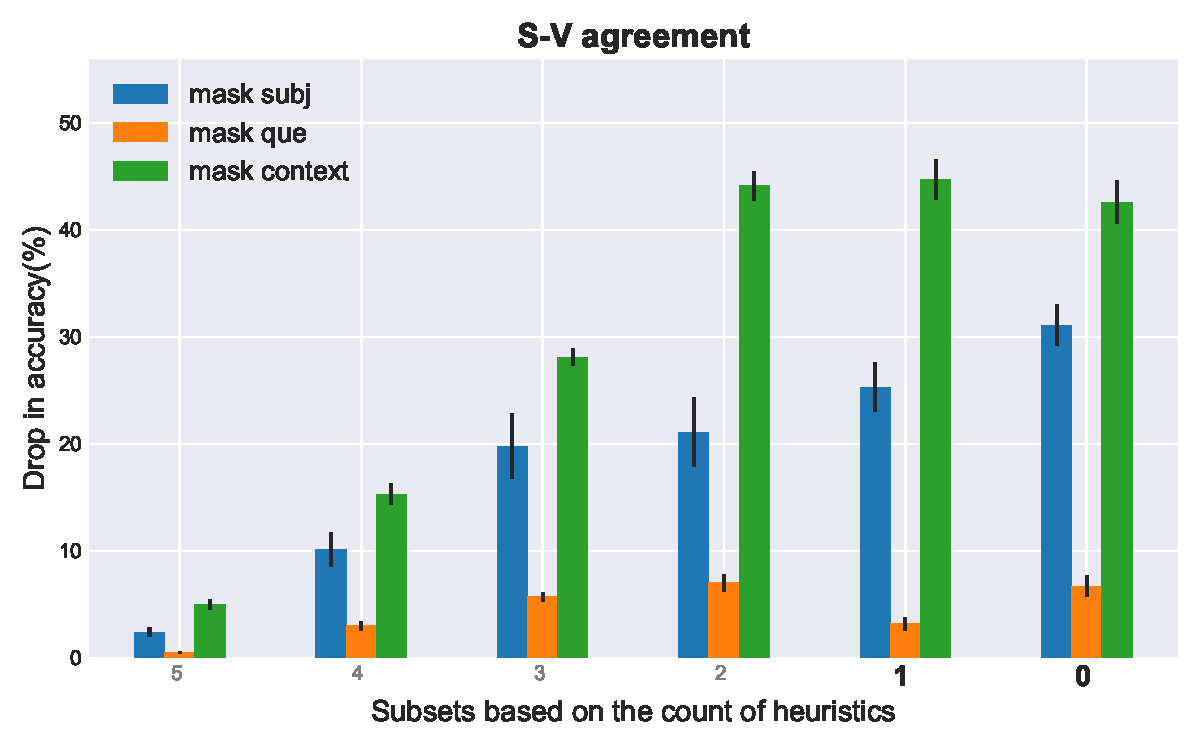
\includegraphics[width=\columnwidth]{figures/causal-subj-v.pdf}}
\scalebox{.95}{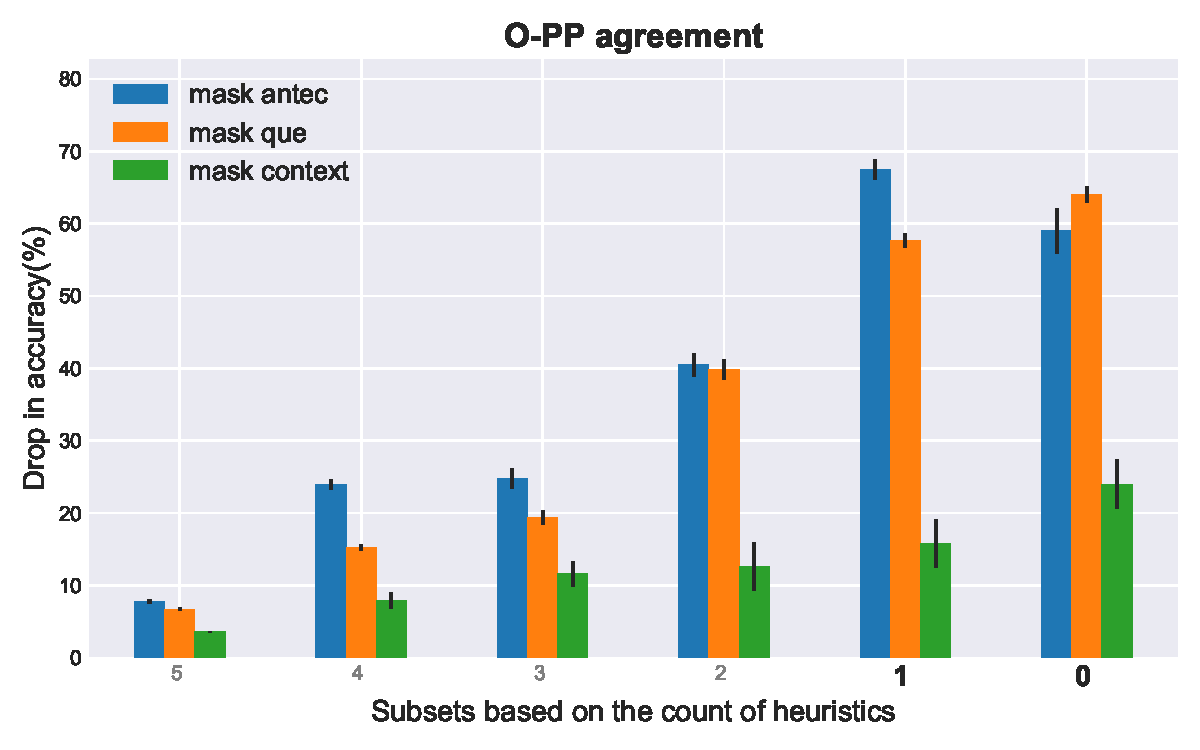
\includegraphics[width=\columnwidth]{figures/causal-obj-pp.pdf}}
\caption{Average causal effect of interventions on Transformer's NA task performance, quantified by drop in accuracy before and after different interventions, and further broken down based on prediction difficulty measured by the number of heuristics. The term \emph{cue} here refers to the antecedent and its modifiers (determiners and adjectives) in O-PP agreement, and to the subject and its modifiers in S-V agreement.} \label{fig:causal_res}
\end{figure} 

\paragraph{Results} In Figure~\ref{fig:causal_res}, we report the changes caused by different interventions, as quantified by the average causal effect. This effect represents the drop in performance on NA tasks for both S-V and
O-PP agreement.\footnote{See the Table~\ref{tab:full_causal_res} in the Appendix for the full results.} These causal effects are further dissected based on task difficulty. As noted in Section~\ref{sec:h_eval_protocol}, our investigation primarily focuses on the more challenging cases (i.e.\ \emph{0}
and \emph{1 heuristic} subsets), which cannot be resolved via surface heuristics and thus provide robust evidence of a model's capacity to capture sentence structure information.


As observed, the
\emph{cue} (i.e.\ the antecedent or subject groups) turns out to be critical
for predicting the corresponding agreement for both types of agreement. Masking these tokens
strongly degrades Transformer's performance on the 0-, 1-heuristic subsets. For the O-PP agreement, we notice a performance drop of over 59\%, and for the S-V agreement, a decline of over 25\%. Interestingly, the impact of other interventions on the two types of agreement displays marked differences. The role of the relative pronoun ``que'' in determining the form of the target verbs in these two agreement phenomena significantly diverges. In the case of O-PP agreement, masking the relative pronoun leads to a significant decrease in prediction accuracy, decreasing by over 57\%. Conversely, it has minimal effect on the prediction of subject-verb agreement, with accuracy decreasing by no more than 7 percentage points. This suggests that that even though the two agreement phenomena exhibit highly similar surface forms and the model encodes agreement information in a similar manner (as detailed in Section~\ref{sec:probing}), the Transformer uses separate agreement mechanisms to handle the S-V and O-PP agreements. This distinction thereby lends support to the linguistically-motivated hypothesis.


Figure~\ref{fig:causal_res} also demonstrates that, for S-V agreement across object relatives, the \emph{context} tokens excluding the \cue and ``que'', contribute more significantly to the model's decision than the subject group tokens (i.e., the subject and its dependents) with which the verb agrees. This indicates that \target receives more agreement information from intermediate tokens than from the direct attention to the nominal subject and its dependent words. This pattern contrasts with the O-PP agreement, where direct attention to the two linguistically-motivated components (i.e., antecedent and ``que'') can induce an over 80\% performance drop, compared to a maximum causal effect of 24\% for context tokens. This surprising observation appears to confirm the findings of \cite{ravfogel-etal-2021-counterfactual}, who suggested that to predict S-V agreement, the model uses information about relative clause boundaries encoded in its representations. To account for this intriguing observation, we hypothesize that while the agreement information is distributed across all tokens in the \emph{context} segment, the relative clause boundary information is vital for the model to determine how to use this information to inflect the main verb. This would clarify why the \emph{context} tokens play such a crucial role in controlling the agreement. However, further experiments are necessary to confirm this hypothesis.
 
\subsection{Conclusion} \label{sec:causal_discussion}
In this section, our objective is to identify which tokens mainly provide the agreement information used by the model to resolve the NA tasks, and further determine whether the usage pattern reflects the distinct theoretical modeling of S-V and O-PP agreement phenomena. To this end, we designed a causal experiment based on self-attention interventions. In this framework, the model performed the NA tasks from Section~\ref{sec:heuristics}, but with a twist: when predicting the \target, we cut the direct attention from the \target to tokens proposed to provide agreement information, based on two hypotheses: the linguistically motivated hypothesis and the linear combination hypothesis (supported by probing results in Section~\ref{sec:probing_location}). The model's post-intervention performance was then compared with the pre-intervention performance, with the performance drop indicative of the causal effect of the intervened tokens.


Our experimental findings reveal a distinct pattern in how Transformers use encoded agreement information across the S-V and O-PP agreements. In the case of O-PP agreement, both the \cue and relative pronoun ``que'' serve as crucial sources of agreement information. In contrast, for S-V agreement across relative clauses, while the \cue 
plays an important role in determining the \target's number, the relative pronoun ``que'' has minimal impact on the model's agreement behavior. This discrepancy aligns with the linguistically motivated hypothesis and resonates with the theoretical linguistic analysis of the two agreement phenomena, supporting the Transformer's representational adequacy for capturing syntactic information. Additionally, this reinforces the findings of~\cite{elazar2021amnesic, hanna-etal-2023-functional}, suggesting that the encoding of linguistic properties, as revealed by probing classifiers, may not necessarily be functionally relevant to the model's predictions. This highlights the importance of transitioning from correlational analysis to causal approaches for a more accurate understanding of model behavior. 

This study also opens up several avenues for future research. A primary focus could be on identifying token positions that provide misleading agreement information, leading to incorrect model behavior. To address this, a more controlled experimental setup is needed: Common error patterns from the model's predictions can be extracted (\S\ref{app:NA_error_pattern}), serving as the basis for creating a template-based evaluation set. Subsequently, the causal framework presented in this section could be applied to individual token positions to identify the sources of the model's erroneous predictions. Additionally, questions persist about the underlying mechanisms that allow the \textit{target} token to obtain precise agreement information from intermediate tokens, as well as how the model encodes and uses information about relative boundaries. These questions present compelling areas for future investigation.


\section{Word order: the impact of positional encoding on NLM's syntactic abstraction capacity } \label{sec:word_order_NA}

In the preceding section, we explored the inner workings of the Transformer language model by applying causal intervention on its self-attention mechanism. Our results indicate that the model is capable of leveraging the hierarchical structure of sentences for nuanced, grammar-based generalization. Yet, one might wonder how a Transformer-based language model can approximate a hierarchical understanding of sentence structure when it processes all tokens simultaneously from linear sequence input. To address this, the current section shifts focus to a critical aspect of language that the self-attention mechanism is not inherently equipped to handle: word order information.


Unlike RNNs, which naturally encode word-order information by sequentially processing input elements, the Transformer model processes all tokens in a sequence simultaneously. As a result, the Transformer does not inherently account for the order of the tokens. This order is crucial for many languages where position encodes grammatical functions. Even in free-order languages, token order remains significant, especially given tokenization into sub-word units, making it essential for tasks like language modeling. 

To address this, the Transformer integrates positional embeddings with token embeddings before feeding them into the self-attention mechanism. As detailed in Section~\ref{sec:auto_transformer}, autoregressive language models use an incrementally applied masked self-attention mechanism, which forces the model to attend only to preceding words. This could make positional embeddings redundant, as observed in recent work~\cite{haviv-etal-2022-transformer}. In contrast, masked language models do not have this inherent order modeling, making positional embeddings the sole source of order information.

This study aims to investigate the role of positional embeddings in language modeling and their impact on the syntactic abstraction capacity of Transformer-based language models. Building on the methodology of ablation studies~\citep{meyes2019ablation}, we perform a targeted ablation experiment that focuses on positional embeddings. We compare the performance of autoregressive Transformer LM with and without positional embeddings, and then we run similar experiments with bidirectional Transformer LM~\citep{devlin-etal-2019-bert}. Our experiment is designed to understand the relationship between the model's ability to abstract syntactic structures and its awareness of token order within a sequence.

\subsection{Positional embeddings in Autoregressive Transformer LM} \label{sec:exp_1_tm_nopos}

\paragraph{Experimental setup} In all our previous experiments, we considered an autoregressive Transformer LM, denoted as $\mathcal{M}$, with the sinusoidal positional embeddings described in \cite{NIPS2017_3f5ee243}, which is the standard setting. To delve deeper into the role of explicit position encoding within Transformer LMs, we consider a variant of this model without positional embeddings, denoted as $\mathcal{M}_{nopos}$. The training process for this position-deprived Transformer LM mirrors that of the original model, using the same training data and the same hyperparameters (\S\ref{app:tm_training}).

To assess the importance of positional embeddings for the language modeling objective itself, we conducted an intrinsic evaluation by comparing the validation set perplexity of the model $\mathcal{M}_{nopos}$ and the original model $\mathcal{M}$. As suggested by~\cite{hu-etal-2020-systematic}, perplexity scores do not always give us a clear picture of a model's syntactic ability. Therefore, we also conduct an extrinsic evaluation by comparing the performance of both models, $\mathcal{M}_{nopos}$ and $\mathcal{M}$, on NA tasks. This evaluation helps us assess the importance of explicit position encoding in the model's syntactic abstraction capacity.

 % for the language modeling objective
\paragraph{Results}  In terms of the perplexity obtained on the validation set, the model without positional embeddings, $\mathcal{M}_{nopos}$, has an average score of 27.2 across five pre-trained instances, which is strikingly close to the score of 27.0 for the original Transformer. This counterintuitive result suggests that explicit positional encoding may not be as crucial as we thought for pre-training the autoregressive Transformer LM. 

When it comes to accuracy on NA tasks, as shown in Figure~\ref{fig:tm_nopos_NA_tasks}, the ablation of positional embeddings surprisingly has a negligible impact. This holds true for both the overall accuracy and the stratified accuracies across subsets of varying difficulty, as determined by our heuristic-based evaluation protocol. Again, this is particularly striking considering the often crucial role of word order in encoding syntactic relationships in languages like French.

A plausible explanation for these surprising results is that the autoregressive Transformer's incremental attention mask, which forces each token to attend only to its preceding tokens, may inherently encode word order information. Although all tokens in a sequence are processed simultaneously, the ability of the model to take into account the predecessors of a given token may effectively allow it to deduce its position within the sequence. We explore this hypothesis in the following experiment. 



\begin{figure}[ht]
    \centering
    \begin{subfigure}[b]{0.49\textwidth}
        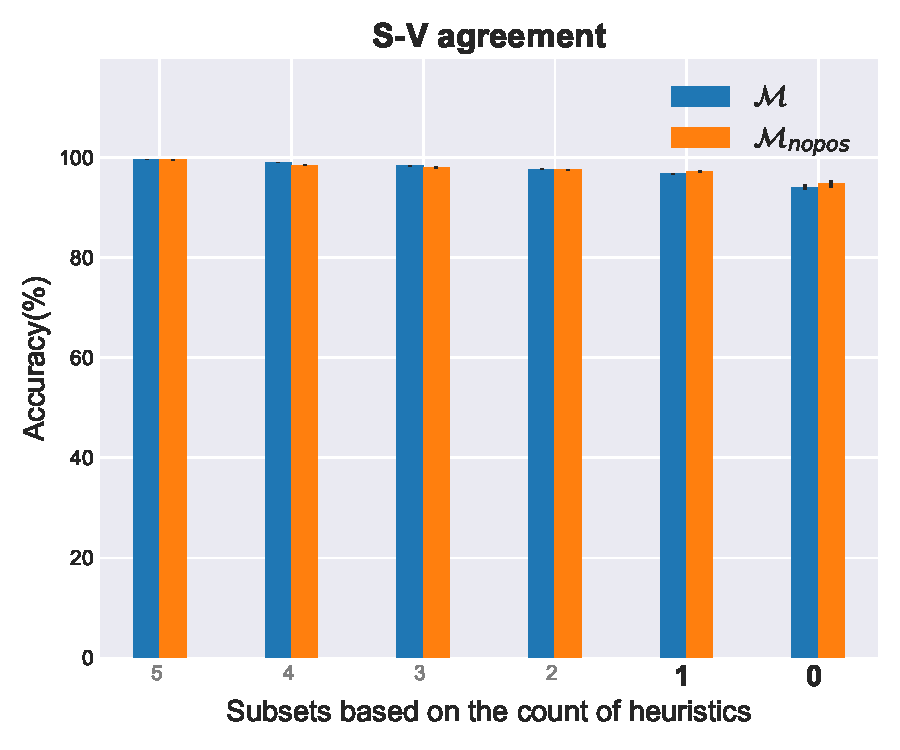
\includegraphics[width=\textwidth]{figures/tm-nopos-subj-v.pdf}
    \end{subfigure}
    \hfill
    \begin{subfigure}[b]{0.49\textwidth}
        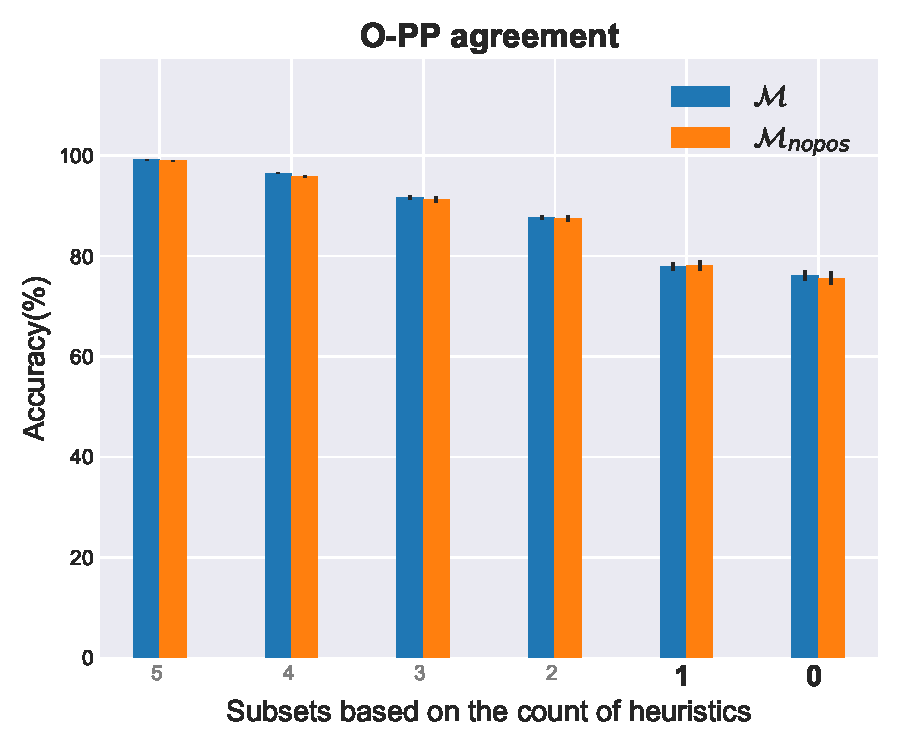
\includegraphics[width=\textwidth]{figures/tm-nopos-o-pp.pdf}
    \end{subfigure}
    \caption{Accuracy comparison of autoregressive Transformer LM on two NA tasks with and without positional embeddings. Detailed scores are reported in Appendix Table~\ref{tab:TM_nopos}. \label{fig:tm_nopos_NA_tasks}}
\end{figure}

 
\subsection{Positional embeddings in masked Transformer LM } \label{sec:exp_2_mlm_nopos}

The previous experiment reveals that an autoregressive Transformer LM deprived of positional embeddings can still perform comparably in language modeling and NA tasks. This leads us to hypothesize that the incremental self-attention mask might be enabling the model to implicitly reconstruct word order position information during the pretraining. To test this hypothesis, we extend our ablation experiment to a Transformer language model trained with a masked language modeling objective \citep{devlin-etal-2019-bert}. Unlike autoregressive language modeling, where the model predicts each subsequent word based on previous tokens, masked language modeling entails predicting randomly masked tokens using both preceding and succeeding context~(\S\ref{sec:lm_tasks}). In this context, positional embeddings serve as the sole source of order information. When removed, the MLM
generates token representations independent of the actual position of tokens in the input sequence, behaving like a bag-of-words model.  The goal here is to investigate whether MLMs can also implicitly learn word order during pre-training without explicit positional embeddings. If they cannot, it would suggest that the incremental attention mask indeed plays a crucial role in the autoregressive model's ability to learn word order information.


\paragraph{Experimental setup} We adapted our generic language model to implement a bidirectional Transformer model, which was then trained using a masked language modeling objective \citep{devlin-etal-2019-bert}. We pre-trained the MLMs both with and without positional embeddings on the same training data (as described in \ref{sec:heuristic_exp_setup}), following the same training process used for the autoregressive models. For each model, we train five different seeds using the optimal hyperparameter configuration.\footnote{Please refer to \S\ref{app:tm_training} for details on the hyperparameters.} We repeat the ablation experiment from \S\ref{sec:exp_1_tm_nopos} to compare the perplexity scores of the pretrained MLMs and their performance on NA tasks in the absence of positional embeddings.

As discussed in Section~\ref{sec:lm_tasks}, perplexity is a standard metric for evaluating autoregressive LMs. This metric is not suitable for models trained using a masked language modeling objective, where a masked token $w_i$ is predicted based on its surrounding context $S_{ \setminus i}$. To evaluate MLMs, we adopt the pseudo-perplexity approach from \cite{salazar-etal-2020-masked}, calculated as the average of the conditional log probabilities $log \mathbb{P}_{MLM}(w_i | S_{ \setminus i})$ for each token. While not comparable to conventional perplexity, it allows for a direct comparison between MLMs. More details can be found in the appendix~\ref{sec:ppl_lm}. 

\begin{figure}[ht]
    \centering
    \begin{subfigure}[b]{0.49\textwidth}
        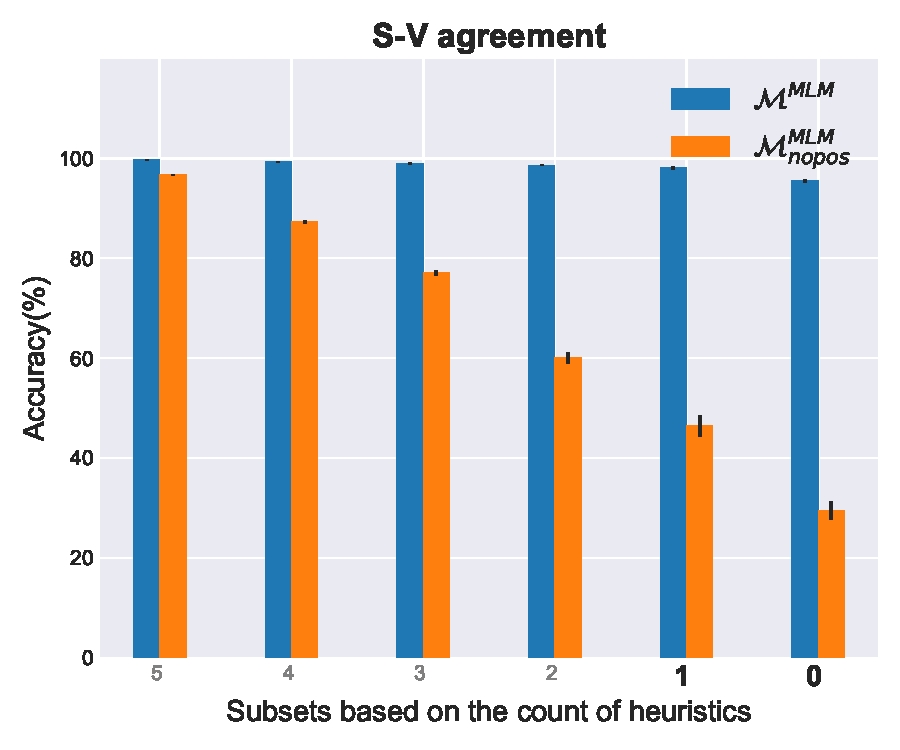
\includegraphics[width=\textwidth]{figures/mlm-nopos-subj-v.pdf}
    \end{subfigure}
    \hfill
    \begin{subfigure}[b]{0.49\textwidth}
        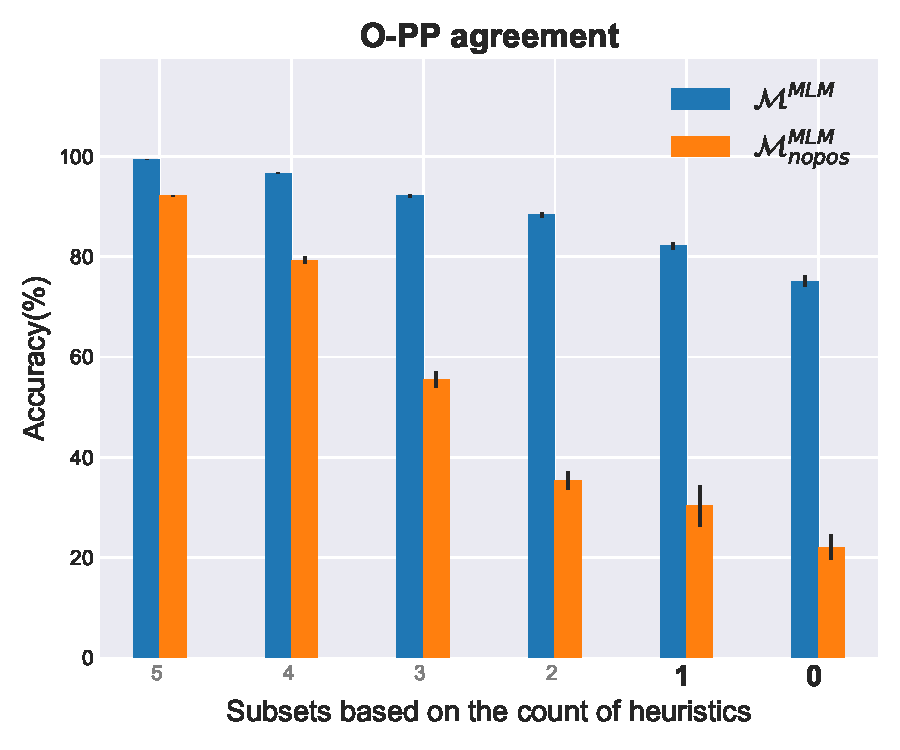
\includegraphics[width=\textwidth]{figures/mlm-nopos-o-pp.pdf}
    \end{subfigure}
    \caption{Masked Transformer LM's accuracy on two NA tasks with and without positional embeddings. Detailed scores are reported in Appendix Table~\ref{tab:MLM_nopos} \label{fig:mlm_nopos_NA_tasks}}
\end{figure}

\paragraph{Results}
Our experiments show a substantial difference in pseudo-perplexity scores between the masked language models with and without positional embeddings. The position-aware MLM converges to a very low score of 5.6, whereas the \texttt{nopos} MLM performs significantly worse, with a score of 57.2. This result aligns with the observations of previous studies such as \cite{sinha-etal-2021-masked} and \cite{haviv-etal-2022-transformer}, which noted that MLMs deprived of explicit position encoding suffer a substantial decline in pretraining task performance.

Regarding the performance on number agreement tasks, as seen in Figure~\ref{fig:mlm_nopos_NA_tasks}, the ablation of positional embeddings leads to a substantial decrease in accuracy across both agreement tasks. Particularly, in the most challenging cases, the performance drop reaches 66\% for S-V agreement and 53\% for O-PP agreement. These findings indicate that explicit position encoding plays a critical role in MLM's syntactic abstraction ability. This, in turn, provides evidence supporting our initial hypothesis concerning autoregressive LM, suggesting that the incremental attention mask may enable it to implicitly reconstruct absolute word position information.



\subsection{Conclusion}
In this study, we have performed a set of positional embedding ablation experiments with both autoregressive and bidirectional Transformer LMs. These models are evaluated based on their performance in language modeling and number agreement tasks, comparing the outcomes of models with positional embeddings against those without. Our results show that the autoregressive language model deprived of positional embeddings (\texttt{nopos}) achieves competitive performance compared to its original counterpart in both the language modeling task and the NA tasks. In contrast, bidirectional language models without positional embeddings experience substantial performance degradation in both language modeling and NA tasks. This stark contrast highlights the critical role positional embeddings play in bidirectional models in identifying token positions. Meanwhile, autoregressive LMs appear to leverage the incremental attention mask to implicitly reconstruct word order information, thereby the absence of explicit position encoding has very little impact on the model's performance.

\section{Conclusion and discussion} \label{sec:conclu_main_projct}
In this chapter, we conducted a contrastive study to explore the core question of my thesis: Does the Transformer language model exploit abstract sentence structures, or does it primarily rely on surface patterns when handling structure-sensitive phenomena? Our primary goals are twofold: to assess the behavioral and representational adequacy of the autoregressive Transformer model in relation to human syntactic processing, and to develop a linguistically-informed framework to enhance the interpretability of this complex model. To achieve this, we use number agreement tasks to explore how the Transformer LM processes two forms of agreement in French: long-distance subject-verb and object-past participle agreements, both involving object relative clauses. While these two types of agreement share superficial similarities in word sequences, their linguistic analyses fundamentally diverge.

Our approach begins with the proposal of a heuristic-based evaluation protocol, which effectively constrains the impact of surface heuristics in conventional number agreement tasks, providing a robust groundwork for our subsequent experiments. In our initial set of experiments, we assessed the ability of an autoregressive Transformer language model to predict these two types of agreement. The results indicate that the model exhibits high predictive accuracy, even under challenging conditions where all surface heuristics fall short. Further control experiments underscore the Transformer's ability to generalize beyond collocational cues and strong frequency biases. Taken together, these results strongly suggest that the Transformer is not merely exploiting surface patterns, but may be capturing some form of abstract sentence structure. This evidence indicates that Transformer meets the first prerequisite --- behavioral-level similarity --- for genuine syntactic generalization.


Building on the strong behavioral performance of the Transformer, we took a more in-depth investigation to assess where syntactic agreement information is located within the model's inner representations, as a measure of its representational adequacy. Our second set of experiments, using a probing approach, reveal that the relevant agreement information is mainly linearly encoded across all tokens between the \cue and the \target. Interestingly, within the contextualized representations, this information is found in a small number of highly correlated dimensions, while also being fuzzily encoded in a redundant manner across the remaining dimensions. Notably, we observe a very similar distribution pattern of agreement information for both types of agreement phenomenon.

To go beyond the limitations of probing, which mainly reveals correlations between encoded information and the model behavior, we introduced a causal framework. This framework relies on counterfactual analysis and involves intervening directly on the model's self-attention mechanism. Our causal experiments provide further evidence that the Transformer model's success is based on linguistically justified cues, consistent with French grammar. Importantly, the abstract structure uncovered by the Transformer model aligns with the distinct theoretical modeling of the two structure-sensitive phenomena we examined. This alignment supports the Transformer's representational adequacy for capturing syntactic information, suggesting that its internal mechanisms are not merely statistically efficient but also linguistically meaningful. Consequently, this lends additional credibility to the potential of the Transformer as an explanatory tool for human syntactic processing. 

 
Additionally, to investigate how Transformer language models approximate syntactic structures from string input, we conducted a set of positional embedding ablation experiments with autoregressive and bidirectional Transformer LMs. We find that explicit position encoding has little impact on the general function and syntactic abstraction ability of the autoregressive LM. This is likely because the model can leverage the absolute word order information from the incremental attention mask. 

Our study represents an initial step towards a deeper understanding of how neural language models function. Our analysis framework, which begins with behavioral syntactic tasks fortified by heuristic-based evaluation, then pairs with linguistic probes, and finally explores through counterfactual analysis via causal intervention, provides a robust methodology to assess the syntactic abstraction capacity of neural language models. Notably, our findings regarding the linguistically motivated distribution of syntactic information in Transformers' representations could extend easily to other linguistic phenomena and languages.

Nevertheless, many questions remain unresolved, such as the precise mechanism by which Transformers track agreement information and how they encode long-distance dependencies from linear word sequences. It is also of interest to explore whether the model can emulate a human-like rule-based generalization to dynamically recombine familiar structures in novel situations. These avenues represent exciting directions for further investigation. Our work thus far only marks the beginning of a rich and exciting journey toward deciphering the complex inner workings of neural language models.